\chapter{Bolund Hill}

\section{abstract}
The recent proliferation of wind energy led in an increased penetration of wind farms in complex terrains. Unlike simple terrains, near surface wind experiences high variation in velocity and enhancement of turbulence in the complex terrains. Local measurement in sparse locations is inadequate to assess such diverse wind profile and application of numerical models has the potential to deliver detailed insight. In this work, the Bolund hill experiment, a rigorous complex terrain field campaign, is used to validate a Large Eddy Simulation (LES) model. The LES model applied is available in the SOWFA solver library developed based on the open-source solver OpenFOAM. A series of precursor LES has been performed to bridge the gap between atmospheric macro scale with terrain induced micro scale and used as a source of turbulent inflow for the Bolund hill LES. The influence of turbulent inflow is compared with a steady inflow LES. The sequential precursor LES found consistent in terms of mean velocity and turbulence stresses. Although, minor differences found for mean wind speed, the TKE of the steady inflow Bolund hill LES is always under-estimated. The precursor inflow fed Bolund hill  LES performed well in areas of nearly flat terrain and have a few scope of improvements in the difficult flow regions such as steep slope and ridges. Due to computational resource limitation, only two hill LES with different turbulent inflow for ten minutes each has been performed, which is statistically inadequate compared to enormous data compiled in the experimental campaign. This study identified the importance of turbulent inflow for complex terrain LES  and established a feasible and optimal approach to generate turbulent inflow through sequential precursor LES. Bolund hill LES resulted in some encouraging results and we identified the areas which need a more careful investigation to improve the overall prediction.


\section{Introduction}
\label{sec:1}

In recent years, the proliferation of wind energy led to the erection of wind farms in complex terrains to take benefit from better wind resources. Complex terrain substantially affects wind velocity and turbulence characteristics particularly in the near-surface region and around bluff bodies. Speed up of mean wind is often found with significant enhancement in turbulence. Hence, good knowledge of wind flow over complex terrains is essential to evaluate wind energy potential, assess structural loads, determine wind turbine design and sitting, and ultimately derive wind farm economics. Measurement from meteorological towers in sparse locations is essential, but not sufficient to reflect the intricate wind profile in complex terrains. Numerical models have the potential to offer insight with high fidelity information in this regard.

Wind flow in complex terrains exhibits diverse phenomenon ranging from flow stagnation, rapid acceleration-deceleration, recirculation-reattachment, vortex shedding, etc. Such micro-scale events occur at higher frequencies (as well as at smaller spatial scales) compared to meteorologic synoptic scale events. To resolve these flow features, the numerical models have to operate in a time accurate manner along with grid resolution in the order of length-scale of these 

Turbulence models like Reynolds Averaged Navier-Stokes (RANS) models are very economical to operate, however, only provide statistically averaged solution. Besides, they are known to be inaccurate in the flow separation-recirculation zones. The Large Eddy Simulation (LES) models provide a viable alternative, which provides an accurate prediction with the trade-off of higher computational cost. LES models only resolve relatively large-scale events and mathematically model the smaller scales, thus can be set to capture flow structures evolving around the complex terrains. Prior to the application with confidence, irrespective of category, any turbulence model need to be validated against experimental measurements.

Over the past three decades, following wind farm sitting in simple terrains, various atmospheric boundary layer flow experiments were performed on terrains with gentle slopes. The main focus of these studies was to derive mean wind profile and turbulence intensity, whereas insight into terrain and flow turbulence interaction was limited. This was partly due to most of the available numerical models was either linear or RANS type model, which do not produce information regarding turbulence structures. 

With growing penetration of wind farms in complex terrains, accurate and high-fidelity information of complex wind flow became important. In recent years, due to the abundance of inexpensive computational resources, application of LES models become feasible. LES models can reproduce spatio-temporally varying turbulent flow, thus higher order and spectral analysis can be performed which is important to understand the effect of turbulence on wind turbine structures. Despite encouraging potentials, performing LES is challenging, because of difficulties in sub-grid-scale model applied (to account for small turbulent scales), specifying appropriate boundary condition particularly the inflow condition, treatment of rough terrain surface, etc. The ``Bolund Experiment''\cite{Berg2011} is a benchmark case for atmospheric boundary layer flow over complex terrain and considered as the validation test case in this study. A LES model from the open-source SOWFA \cite{Churchfield2012, Churchfield2013} solver library is used to reproduce the experimental campaign over the Bolund hill. The experiment description, review of the previous validation studies and details of the current LES model validation are elaborated in the subsequent sections.


\section{The Bolund Hill experiment}
\label{sec:2}

\subsection{Topology}
\label{subsec:2.1}

The experimental campaign is performed on an isolated hill in Bolund Peninsula, located north of Riso campus of DTU in Roskilde Fjord, Denmark during three winter months of 2007-2008\cite{BolundProjectWeb}. The Bolund hill is a naturally formed island of an approximate dimension of $150 m$ length in the west-east direction, $100 m$ width in the south-north direction, and $11 m$ in height. The hill is mostly flat and surrounded by a narrow beach. On the west side, it has an almost vertical escarpment with some overhanging portion. The other sides have a moderate slope with rounded crest. Being located in a bay, the hill is ringed by water in all except east direction where a narrow isthmus connects the hill with the mainland. The figure \ref{fig:contour} depicts a contour map of the Bolund hill terrain and measurement mast locations.

%
\begin{figure}
    \centering
    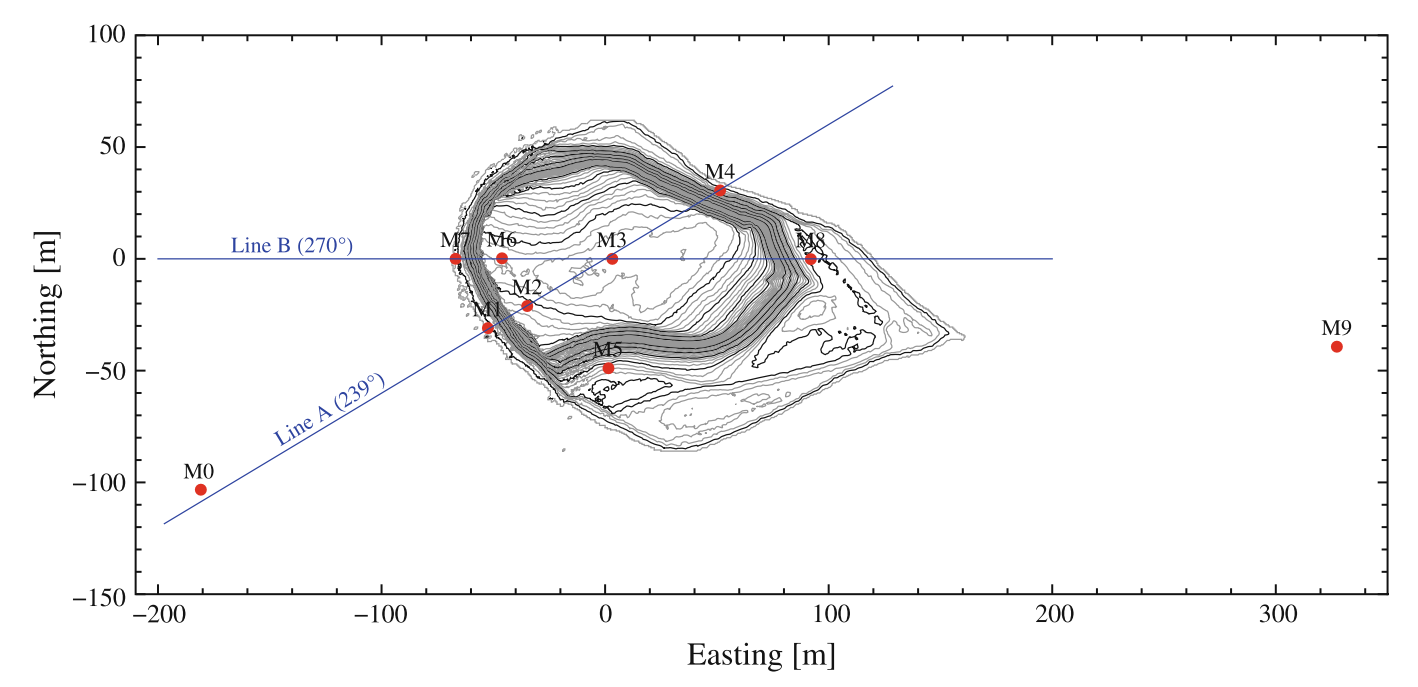
\includegraphics[width=0.75\textwidth]{./contour-wMast.png}
    \caption{Countour map of the Bolund hill in 0.25m interval. The masts (marked in red dots) are located along two transects A and B. The mast M3 denotes the center point of the hill [image reproduced from Bechmann et al. \cite{Bechmann2011}] \label{fig:contour}}
\end{figure}
%

The Bolund hill center is defined arbitrarily on top of the hill to serve as the local reference, which is also the position of mast M3. The measurement mast M0 is placed approximately 181 m west, 100 m south of hill center out at sea (on a floating platform). On the Bolund hill, measurement masts are placed along two lines to capture flow from two predominant wind directions. Four masts (M1, M2, M3, M4) are aligned with Line A with an angular orientation of $239^o$ and four more masts (M3, M6, M7, M8) forms the Line B of $270^0$ angle. The mast M5 is placed in the due south on the beach and mast M9 is placed approximately $327 m$ east and $39 m$ south on a small beach, which is south of the isthmus.

For ease of simulation, only the westerly wind ($270^0$) is considered for the validation study. The mast M0 is assumed to be placed in sufficient upstream distance to measure the incoming wind profile. The mast M9 will serve to examine downstream wind affected by the bluff shape of the hill. On each mast, multiple anemometers (cup/sonic) are placed at different heights to record the wind profile. Two temperature probes at different height were placed on each mast M0 and M9 to determine the atmospheric stability condition. In the experiment, data sets are collected at $20 Hz$ sampling rate in $10$ minute blocks for all probes. For the current study, data sets with average wind speed exceeding $5 m/s$ and $|1/L_{MO}| < 0.004 m^{-1}$ have been selected for validation, where $L_{MO}$ is the Monin-Obukhov length (eq. \eqref{eq:MO}). 

The westerly wind experiences an approximately $7\, km$ fetch over the calm bay which is characterized by a small roughness height of 0.0006 m \cite{Berg2011}. Such near-perfect incoming flow condition provides a well-defined quantitative description of incoming flow and it is crucial for boundary condition implementation in the numerical models. Except for the sandy beach and near-vertical escarpment, the Bolund hill is mostly covered with grass and characterized by a uniform roughness length of 0.015 m \cite{Berg2011}. In the field experimental campaign, a maximum 30 \% speedup is found associated with 300 \% enhancement of turbulence intensity \cite{Berg2011}. It implies that the best site for the erection of wind turbines to maximize energy harness have to bear a penalty of increased structural fatigue loads. For the westerly wind, the Bolund hill also features a transient recirculation zone at the escarpment edge and downstream flow deceleration in the eastern slope.

%
%
%
\subsection{Scale effects}
\label{subsec:2.2}
%
The physical shape of the Bolund hill represents a scaled down form of a typical wind turbine site in complex terrain. Hence, computational resources required for Bolund hill simulation will be much smaller than a realistic complex terrain e.g. a mesa hill. However, the scale effects shall be accounted before inferring any decision made from Bolund hill simulation. Berg et al. \cite{Berg2011} suggested a typical mesa hill of $10-30$ times in all dimensions and aerodynamic surface roughness length.

According to S. Pope \cite{pope2000tf}, Reynolds number similarity implies Reynolds number independent flow solutions and is essential for turbulence models such as LES. In the present study, Reynolds number is defined based on the hill height $h$ and the free-stream velocity $U$. For Bolund hill with $U \approx 10 m/s$, $Re_{Bolund} \approx 10^7$ and for the same characteristic velocity over the mesa hill, $Re_{mesa} \approx 10^8$. Lim et al. \cite{Lim2009} conducted a series of wind tunnel experiments of flow over bluff bodies in a turbulent boundary layer with concentrated vortex motion and studied flow Reynolds number up to $10^6$. Even at such high Reynolds numbers variation observed in surface pressure and near surface speed with the change of Reynolds number. Although the Bolund and mesa hill Reynolds numbers are even higher of a different flow type, the Reynolds number dependence cannot be ruled out completely.

Influence of atmospheric stability and boundary layer height $z_i$ is also important when scaling up Bolund to the mesa hill. The Monin-Obukhov length determines the height of significant surface influence within the boundary layer and defined as
%
\begin{equation}
\label{eq:MO}
 L_{MO} = - \frac{u_{*}^3}{\kappa (g/ \theta) \overline{w^\prime \theta^\prime}},
\end{equation}
%
where the friction velocity is defined by $u_* = \left[ \overline{u^\prime w^\prime} + \overline{v^\prime w^\prime}\right]^{1/2}$. Here, $u\, v \, w$ are the averaged axial, lateral and vertical components of the wind velocity vector respectively, $\theta$ is the potential temperature and the primed quantities are fluctuations around these values. The $\overline{...}$ represents the ensemble average operator. $\kappa=0.4 $ denotes the von-Karman constant and $g$ is the gravitational acceleration constant.

For Bolund experiment, the hill height is much smaller than the temperature inversion height (boundary layer depth) $z_i$ and the Monin-Obukhov length $L_{MO}$. Therefore flow perturbations induced by the bluff hill expected to dominate over perturbations caused due to atmospheric instability \cite{Berg2011}. So irrespective of atmospheric stability condition, the atmosphere can be approximated as neutral. However, such assumption may not be applicable for the mesa hill. In a neutral atmosphere with high wind speed or in an unstable atmosphere where boundary layer height $z_i$ is very high, stability effects can be neglected. In the case of the stable atmosphere, where the boundary layer depth $z_i$ is usually low (comparable to mesa hill height), strong effects of stratification are expected and generalization from Bolund to mesa hill fails \cite{Berg2011}. In the current study, experimental measurements recorded only in a neutral atmosphere are used for LES model validation.

The influence of Coriolis force shall be accounted as well. For vertical direction, the Ekman depth has an approximate size of atmospheric boundary layer height. Thus, change of wind direction with height may influence the mesa hill flow at least in a stably stratified atmosphere. The height of Bolund hill is much smaller than the Ekman depth and hence Coriolis effect in the vertical direction can be neglected. To estimate influence in horizontal direction, the Rosby number ($Ro = U/fL$, where $f \approx 10^{-4} s^{-1}$ for mid-latitudes has been taken into account. For Bolund hill, $Ro \approx 660 >> 1$ and Coriolis effect on the wind can be overlooked. On the other hand, for mesa hill, $Ro \approx 60 > 1$ and Coriolis effect may become significant. Therefore, numerical simulation of Bolund hill can be performed for the neutral atmospheric boundary layer without accounting for the Coriolis force effect. 


\section{Previous validation studies}
\label{sec:3}

To date, a number of RANS and LES simulations have been performed for the Bolund Experiment. During 2009, a blind comparison workshop was organized to compare 88 different validation studies performed with physical models as well as various types of linear and CFD simulation models \cite{Bechmann2011}. A few more  studies have also been published since then.

In terns of mean velocity speedup, the RANS models produced a $10-20\%$ error on average (Berg et al. 2 eq. $15.1\%$ \cite{Berg2011}, Berg et al. 1 eq. $17.2\%$ \cite{Berg2011}, Prosthaopoulos et al. $10.3\%$ \cite{Prospathopoulos2012}). For the turbulent kinetic energy (TKE), the error is about $50 \%$ (Berg et al. 2 eq. $47\%$ \cite{Berg2011}, Berg et al. 1 eq. $45\%$ \cite{Berg2011}. Prospathopoulos et al. concluded that RANS models can not reveal the small-scale intermittent behavior such as flow recirculation over the edge of escarpment-top \cite{Prospathopoulos2012}.

On the other hand, some LES models demonstrated slight improvement over the RANS models. Deviation of the mean velocity is found in the range of $10-20\%$ (Conan et al. $11\%$ \cite{Conan2015}, Diebold et al. $12.1\%$ \cite{Diebold2013}, Bechmann et al. $17.3\%$ \cite{Bechmann2011}) and for TKE in $20-50\%$ (Conan et al. $20\%$ \cite{Conan2015}, Bechmann et al. $48\%$ \cite{Bechmann2011}). 
Significant deviations were mainly observed in the near-surface regions and the prediction got better at higher elevations.
 
Prescribing the appropriate turbulent inflow is crucial and challenging for atmospheric boundary layer simulation. In the case of RANS models, average velocity and turbulence parameters (e.g. TKE) are prescribed for the inlet boundary condition. However, LES models require realistic spatio-temporally varying turbulent inflow. Precursor simulations and boundary layer recirculation (also called recycling method) \cite{Conan2015,Vuorinen2015} are commonly used methods to generate turbulent inflow for LES simulations.

In terms of mesh generation, two approaches are being mostly used. The terrain following meshing approach uses cells that follow the terrain surface and extrude in the vertical direction. From a meshing perspective, preparation of a terrain-following mesh over complex topography is challenging but provides the option to resolve the near-surface boundary layer and was applied in simulations performed by Conan et al.\cite{Conan2015} and Bechmann et al.\cite{Bechmann2011}). The other approach is the Immersed Boundary Method (IBM), which superimposes the terrain surface into a Cartesian grid and solves for the computational cells above the terrain only (e.g. Jafari et al. \cite{Jafari2012}, Diebold et al.\cite{Diebold2013}). Mesh generation in IBM is fast and usually require fewer grid cells. However, its' capacity to resolve the near-surface boundary layer is somewhat limited. 

Since the terrain surface is rough, the flow boundary layer can't be resolved down to the surface. In practice, wall models are used to prescribe shear stress at the surface to reproduce the logarithmic law of wall region of the mean boundary layer velocity profile. The accuracy of the wall model is important particularly in regions of abrupt surface roughness change (here calm sea and grass covered hill)) and flow separation-recirculation. In the case of complex terrain, local flow variation is present in smaller spatial and temporal scale compared to typical simple terrain simulations and so a finer mesh resolution is recommended (Berg et al. \cite{Berg2011}).

\section{LES model description}
\label{sec:4}

In this work, the Simulator for On/Offshore Wind Farm Applications (SOWFA) which is an OpenFOAM \cite{weller1998OpenFOAM} based solver library developed at the U.S. Department of Energy’s National Renewable Energy Laboratory (NREL)\cite{Churchfield2012, Churchfield2013} is used for the Bolund hill simulation. SOWFA is based on the incompressible Navier-Stokes equations for atmospheric/wind farm large-eddy simulation (LES) that incorporates the Boussinesq approximation for buoyancy and adopts a PIMPLE (PISO/SIMPLE) algorithm for the pressure-velocity coupling. 

The governing equations for mass conservation is
%
\begin{equation}
\label{continuty}
\ddx{\Ua{i}}{i} = 0,
\end{equation}
%
and the momentum conservation equation is
%
\begin{equation}
\label{momentum}
\ddt{\Ua{i}} + \ddx{\Ua{i} \, \Ua{j}}{j} = - \frac{1}{\rho_0} \ddx{\av{p}}{i} + \rho_b g_i - \ddx{\tau_{ij}}{j} -2 \epsilon_{i3k} \Omega \Ua{k},
\end{equation}
%
where viscous fluxes are neglected due to the hign Reynolds numers of ABL flow. The energy conservation equation can be expressed as the potential temperature transport equation and expressed as
%
\begin{equation}
\label{potTemp}
\ddt{\av{\theta}} + \ddx{\Ua{j} \, \av{\theta}}{j} = - \ddx{\tau_{\theta i}}{i}.
\end{equation}
%

In the governing equations above, the overline $\av{...}$ denotes the LES filtering operator and $\Ua{i}$ is the component of the resolve velocity vector in the $x_i$ coordinate direction. The modified pressure is considered as the deviation from the hydrostatic pressure $p = p - \rho_{0}gh$ where $\rho_{0}=1$ is a reference density which is constant in the flow. The Boussinesq approximation considers density as a variable only in the gravitational term. Here, $\rho_b$ is a scalar that dictates the sign and strength of the buoyancy force and computed by 
%
\begin{equation}
\label{rhoB}
\rho_b = 1 - \beta \left(\av{\theta} - \theta_0 \right) = 1 - \left( \frac{\av{\theta} - \theta_0}{\theta_0} \right),
\end{equation}
%
where $\beta$ is the thermal expansion coefficient, $\av{\theta}$ is the resolved scale potential temperature and $\theta_0$ is a reference temperature. The term $2 \epsilon_{i3k} \Omega \Ua{k}$ accounts for Coriolis effect where $\epsilon_{i3k}$ denotes the alternating unit tensor, $\Omega$ is the planetary rotation rate vector at the point of interest on the planet (a latitude dependent quantity) and $g_i$ is the gravitational constant vector.

In LES, the sub-grid-scale (SGS) stress $\tau_{ij}$ and SGS temperature flux $\tau_{\theta i}$ quantities are modeled. The SGS values are usually multiple order of magnitude larger than molecular viscosity/diffusivity and ignored in this LES model. The majority of turbulence models rely upon the linear eddy-viscosity (Boussinesq) assumption that relates the SGS stress to the resolved-scale strain by
%
\begin{equation}
\label{sgsStress}
\tau_{ij}^D = -2 \nu_t \av{S}_{ij},
\end{equation}
%
where $\nu_t$ is the turbulence/eddy viscosity, $\tau_{ij}^D$ is the deviatoric part of the SGS stress and $\av{S}_{ij} = \half \left( \ddx{\Ua{i}}{j} + \ddx{\Ua{j}}{i} \right)$ is the resolved scale strain. Similarly, the SGS temperature flux can be expressed as
%
\begin{equation}
\label{sgsTempFlux}
\tau_{\theta i} = -\frac{\nu_t}{Pr_t} \ddx{\av{\theta}}{i},
\end{equation}
%
where $Pr_t$ is the turbulent Prandtl number. Following the equations \eqref{sgsStress} and \eqref{sgsTempFlux}, the $Pr_t$ is a flow specific parameter which must be prescribed and the eddy viscosity $\nu_t$ have to be defined. Smagornisky \cite{smagorinsky1963LES} devised one of the earliest model for $\nu_t$:
%
\begin{equation}
\label{Smagornisky}
\nu_t = \left(C_s \av{\Delta} \right)^2 \av{S}, \quad \av{S} = \left(2 \av{S}_{ij} \, \av{S}_{ij} \right)^\half,
\end{equation}
% 
where $C_S$ is a model constant, $\av{\Delta}$ is the characteristic LES filter length tied to mesh resolution. Here we adopt the Lagrangian averaged scale invariant dynamic Smagornisky model of Meneveau et al.\cite{MeneveauLagDynSGS1996}. The model constant is calculated as in the conventional dynamic Smagorinsky model
%
\begin{equation}
\label{CsModelAvg}
C_s^2 = \frac{\avT{ M_{ij} L_{ij}}} {\avT{M_{kl} M_{kl}}},
\end{equation}
%
but the averaging is performed along flow streamlines and the averaged quantities are called $\mathcal{I}_{LM} = \avT{ M_{ij} L_{ij}}$ and $\mathcal{I}_{MM} = \avT{ M_{kl} M_{kl}}$. The averaging is achieved by solving transport equations
%
\begin{equation}
\label{ILM}
\ddt{\mathcal{I}_{LM}} + \av{U}_j \ddx{\mathcal{I}_{LM}}{j} = \frac{M_{ij}L_{ij} - \mathcal{I}{LM}} {\theta^* \av{\Delta} \left(\mathcal{I}_{LM} \mathcal{I}_{MM} \right)^{-1/8} },
\end{equation}
%
and 
%
\begin{equation}
\label{IMM}
\ddt{\mathcal{I}_{MM}} + \av{U}_j \ddx{\mathcal{I}_{MM}}{j} = \frac{M_{ij}M_{ij} - \mathcal{I}{MM}} {\theta^* \av{\Delta} \left(\mathcal{I}_{LM} \mathcal{I}_{MM} \right)^{-1/8} },
\end{equation}
%
where $\theta^* = 1.5$ is a model constant. The Smagorinsky constant $C_S$ values are bounded between $0.07-0.14$ in this study.


Because of the rough terrain surface, LES models can't resolve the viscous sub-layer, instead, wall models are used to prescribe shear-stresses where the computational node (cell-center or vertices) next the surface is placed in the logarithmic region of the boundary layer. The Schumann-Grotzbach model \cite{Schumann1975,Grotzbach1977} is used to specify surface-normal shear stresses and all other components are set to zero. The SGS stress at the wall is expressed as
%
\begin{equation}
\label{SchumannGrotzbach}
\tau^{wall}_{ij} =\left\{ \begin{array}{ll}
 -u^2_* \frac{\av{U_i}(z_1)}{\vert \avT{\av{U_i}(z_1)} \vert},& \mbox{i= 1,2; j=3,} \\
 0, & \mbox{otherwise.}\end{array} \right.
\end{equation}
%
where it is assumed that $i=1,2$ refers to the surface parallel coordinates and $j=3$ refers to the wall normal coordinate.


\section{LES simulation results}
\label{sec:5}

\subsection{Generation of turbulent inflow data}
\label{subsec:5.1}

Flow behavior in a time-resolved simulation such as LES is influenced by boundary conditions, particularly by the inflow condition. Flow turbulence can be described in terms of pseudo-random coherent motions of a wide range of spatial and temporal scales superimposed on some “mean flow” \cite{Tabor2010LesInflow}. In the case of atmospheric boundary layer flow, larger flow scales are determined by meteorologic synoptic events or the terrain geometry (e.g. surface features) and the smallest scales are determined by fluid viscosity. Since LES resolves the relatively large-scale fluid motions only, simulation inflow must bear relevant flow scales in a coherent manner. The precursor simulation method is a well-known approach, where a separate LES of an equilibrium turbulent flow is performed to generate a library of turbulent flow data which can be introduced as inflow to another LES. Precursor data library can preserve turbulence scales with proper spatial and temporal correlation, and correct turbulence kinetic energy spectrum.

In the current study, westerly wind ($270^0$) in a neutral atmospheric boundary layer is investigated. A precursor simulation of dimension $L\times W\times H = 3000 m \times 3000 m \times 1000 m$ with a flat terrain of recommended calm sea surface roughness of $z_{0} =0.0006 m$ is performed. The domain is aligned in $+x$ as the east, $+y$ as the north and $+z$ as the vertical direction. Coriolis forces have been neglected as discussed in section \ref{subsec:2.2}. In the horizontal plane, a uniform grid resolution of $\Delta x = \Delta y = 10 m$ is applied. In the vertical direction, near surface resolution is kept $\Delta z_{terrain} = 5 m$ which gradually grows up to $\Delta z_{max}= 15 m$ at the top-most edge. The whole precursor Cartesian grid consists of $300 \times 300 \times 100 = 9 \times 10^6$ hexahedral cells. The east-west and north-south boundary pairs are considered as periodic for all variables. The Schumann-Grotzbach model \cite{Schumann1975,Grotzbach1977} for wall shear stress is applied to the surface and the required velocities at the first cell centers are averaged horizontally to estimate the ensemble averaged velocity. Due the use of a stress BC at the surface, specifying a surface velocity is not strictly necessary but the test filtering method used in the dynamic model relies o surface velocity values. Following the SOWFA standard, the velocity at the surface is obtained by linear extrapolation from the 1st and 2nd cell-center values. Flux-based boundary conditions are applied for velocity $\mathbf{U}$ and modified pressure $p_{rgh}$ in the top boundary which allows for inflow and outflow across the boundary. All other variables are declared as ``zero'' gradient Neumann condition at the top boundary.

The velocity field is initialized with some periodic perturbations superimposed on a mean velocity profile prescribed based on the logarithmic law of the wall. A constant potential temperature of $288K$ is prescribed throughout the domain. The \textit{ABLSolver} from the SOWFA \cite{Churchfield2012, Churchfield2013} library is used to execute the simulation for $17,000 s$ to achieve flow equilibrium and then velocity field is recorded as sample-planes in the east boundary for $2,000 s$ to build the turbulent inflow library. In these planes, vertex values of the instantaneous velocity are stored which are obtained by a linear interpolation from the face centers and the BC. 
%
\begin{figure}[htb]
\centering   %%% not \center
	\subfloat[Instantaneous streamwise velocity $U_x$]{\label{fig:CP-Domain}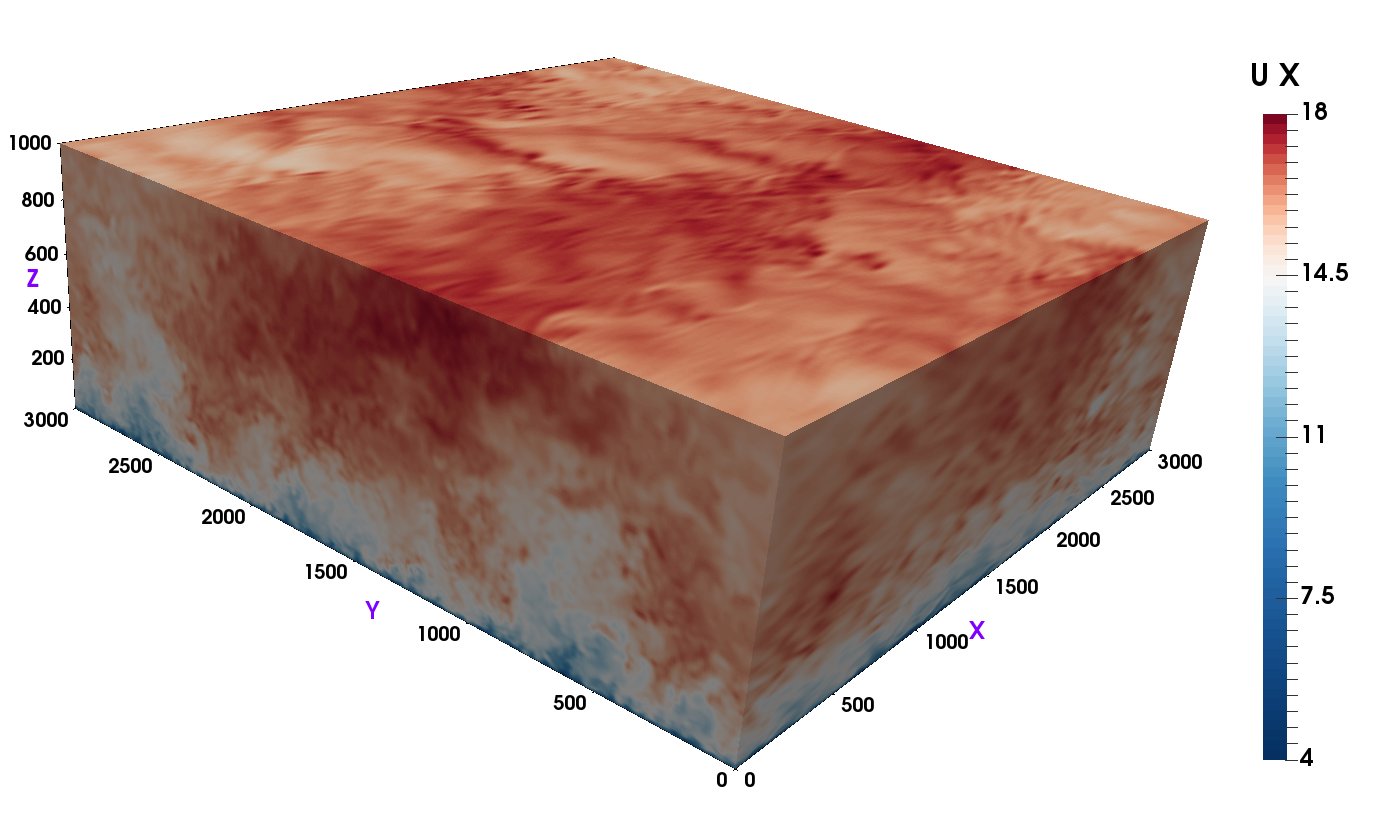
\includegraphics[width=0.55\textwidth]{CoarsePre/precursorVelocity_2.png}}
	\quad
	\subfloat[$U_x$ at $Z_{agl} = 500 m$ plane]{\label{fig:CP-Slice}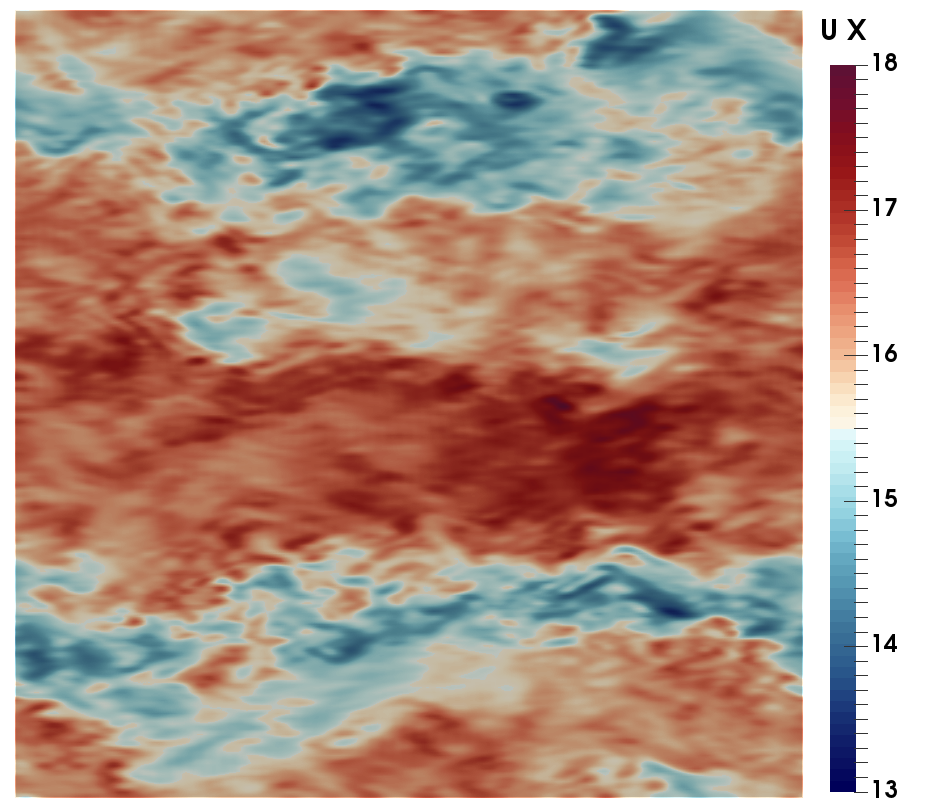
\includegraphics[width=0.35\textwidth]{CoarsePre/Ux_500m_17000s_newcolorscale.png}}
\caption{Precursor simulation over a flat-homogeneous terrain of surface roughness $z_{0} =0.0006 m$.}
\label{fig:CP}
\end{figure}
%

Figure \ref{fig:CP-Domain} illustrates the instantaneous streamwise velocity $U_x$ field of the precursor domain where complex-correlated turbulent flow structures are evident and the figure \ref{fig:CP-Slice} depicts the instantaneous streamwise velocity in a plane $500m$ above the ground ($Z_{agl} = 500 m$). Here, the presence of very long (almost as long as the domain) alternating high and low-velocity streaks are observed. One possible reason for such features could be that the precursor domain is not long enough to allow decorrelation of these very long structures which are cycled back to the domain due to the periodic boundary condition in the streamwise direction.

Fang et al. \cite{Fang2015} conducted a neutral ABL simulation of dimension $L\times W\times H \approx 100,000 m \times 12,500 m \times 1000 m$. The authors observed that the majority of the flow streaks are larger than $5,000m$ (which is larger than present domain extension). They also discovered the presence of very large-scales motions (VLSMs) as long as $20,000 m$ in streamwise and $500 m$ in cross-stream direction. The contribution of structures larger than $10,000 m$ to the resolved kinetic energy and shear stress are found to be up to $27$ and $31\%$ respectively, which is significant. Hence, use of a precursor domain of such large size in the present study seems necessary but infeasible due to enormous computational cost involved. 

The vertical grid resolution of the precursor domain is in the range of $5-15 m$, which also indicates the lower limit of the turbulence structures resolved by the precursor simulation. Since the Bolund hill is about $11m$ high, relatively finer turbulence structures are necessary to observe flow turbulence and hill geometry interaction. Hence, a second precursor simulation with finer resolution is performed using the inflow library from the preceding ``coarse'' precursor and is termed ``fine'' precursor hereafter.

The fine precursor domain has a dimension of $L\times W\times H = 500 m \times 500 m \times 200 m$ with horizontal resolution of $\Delta x = \Delta y = 2m$ and a vertical resolution ranging from $\Delta z_{terrain} \approx 1 m$ (at the surface) to $\Delta z_{max} \approx 4 m$ (at the top). The Cartesian mesh consists of $250 \times 250 \times 100 = 6.25 \times 10^6$ hexahedral cells which are overall about $5$ times smaller in each dimension than the coarse precursor cells. The domain alignment and surface roughness remained unchanged. The flow field variables are initialized from the coarse precursor fields and time-varying turbulent inflow velocity from the coarse precursor is prescribed on the inflow (west) boundary. The recorded instantaneous velocity at the vertices of the coarse precursor is linearly interpolated in space to the fine precursor inlet face centers. Linear interpolation is also used for time as the fine precursor uses a much smaller time step than the coarse precursor. 

The velocity boundary condition at the outflow (east) boundary is specified as ``zero'' gradient Neumann condition and the modified pressure $p_{rgh}$ is prescribed as fixed value ``zero'' Dirichlet condition. A filtered flux-based boundary condition for $\mathbf{U}$ and ``zero'' gradient condition for $p_{rgh}$ is applied in the north, south and top boundaries. Boundary conditions for the surface are kept same as in the coarse precursor. 

The fine precursor contains several cells within one coarse precursor cell (cell center located at $Z_1^{coarse}$). When the inflow data from the coarse precursor is interpolated to the fine precursor inlet face centers, the surface velocity of the coarse precursor would be the lowest value for the linear interpolation and the upper value would correspond to the value obtained from the top face center of the first coarse precursor cell. However, the surface velocity in the coarse precursor is obtained by a linear extrapolation from the 1st and 2nd cell-center values in the surface normal direction and thus does not follow a logarithmic law. Hence, simple linear interpolation of the coarse precursor inflow data will lead to a large error. To avoid this issue, a modified interpolation process is introduced and portrayed in the figure \ref{fig:PreInterp}. 
%
\begin{figure}[htb]
\centering   %%% not \center
	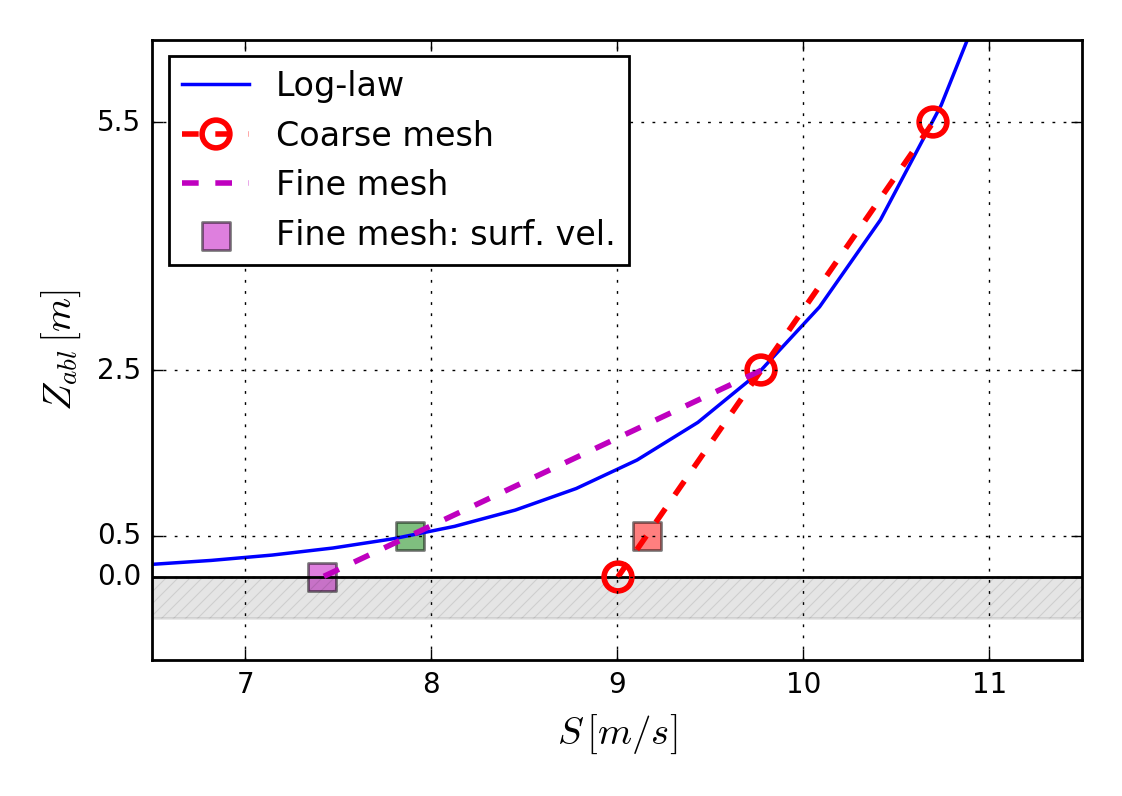
\includegraphics[width=0.5\textwidth]{CPvsFP/PrecursorVelInterpolation.png}
\caption{Modified linear interpolation for coarse to fine precursor projection in the near-surface region}
\label{fig:PreInterp}
\end{figure}
%

In figure \ref{fig:PreInterp}, the ground level $Z_{abl}=0$ is marked by a hatched line and log-law of wall is marked by the solid blue line. Here, the red dashed line depicts the velocity profile approximated by the coarse precursor. If this profile is passed on to the fine precursor, all interpolated values between the surface and $Z_1^{coarse}$ will be significantly larger (e.g. red square marker) than the expected logarithmic profile following values. Hence, the surface velocity of the coarse-precursor inflow library has to be modified (magenta square marker) such that the linear interpolation will provide the correct log-law value (green square) when time averaged. In the presence of multiple cell-centers, all values will follow the modified interpolation path (dashed magenta line) which ensures less error than the primitive interpolation path (red dashed line). Thus, a better near-surface velocity profile is obtained for the inlet boundary of the fine precursor. 

In the fine precursor LES the same \textit{ABLSolver} solver is used and the simulation is first run for $200 s$ to allow for flow evolution. Then, the velocity field is recorded for $1800 s$ on the east boundary to build the second inflow library which will be modified (following the interpolation depicted in fig. \ref{fig:PreInterp}) and fed into the Bolund hill simulation later. Figure \ref{fig:FP} illustrates a comparison between the coarse (left) and fine precursor (right) results of the instantaneous streamwise velocity in a $Z_{agl} = 10 m$ plane at the same time as if they are simulated together. The coarse precursor (fig. \ref{fig:CP-Ux}) represent a plane of the same dimension of fine precursor from the $2500 m$ to west boundary ($3000 m$). The larger scale flow structures in the coarse precursor quickly introduce smaller scale structures along the downstream in the fine precursor (fig. \ref{fig:FP-Ux}). 


%\textcolor{red}{it was not clear to me how the two pictures connect together?}
 
%
\begin{figure}[htb]
\centering   %%% not \center
	\subfloat[Coarse Precursor]{\label{fig:CP-Ux}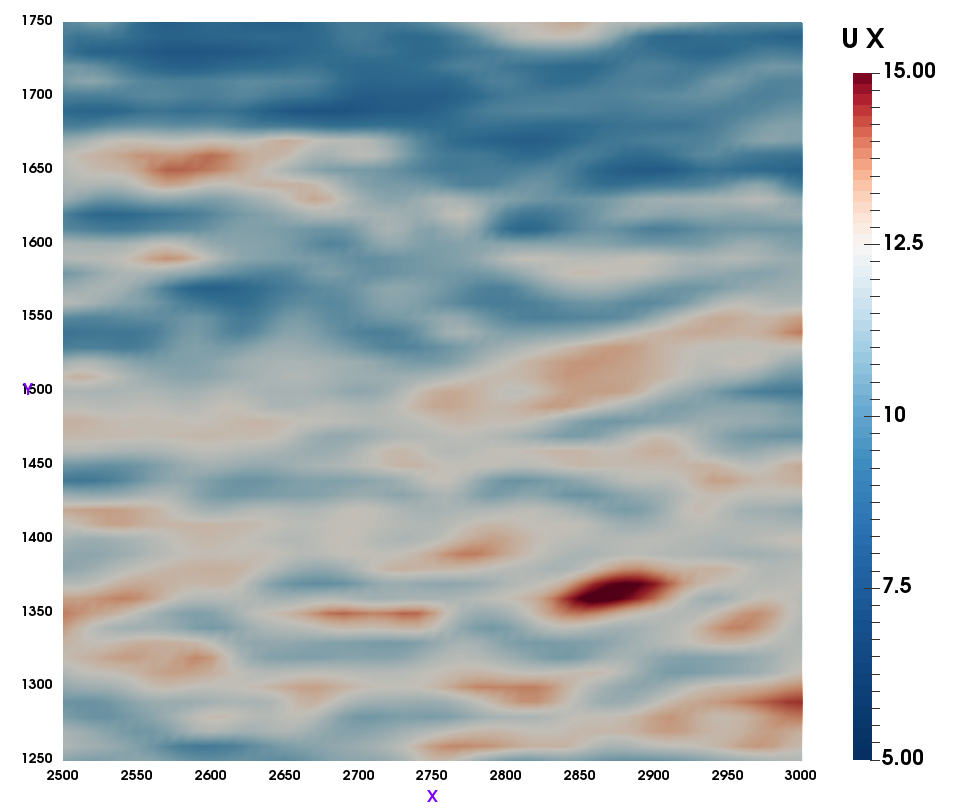
\includegraphics[width=0.46\textwidth]{CoarsePre/finePrePlaneslice_rightside_Ux_z=10m.png}}
	\quad
	\subfloat[Fine Precursor]{\label{fig:FP-Ux}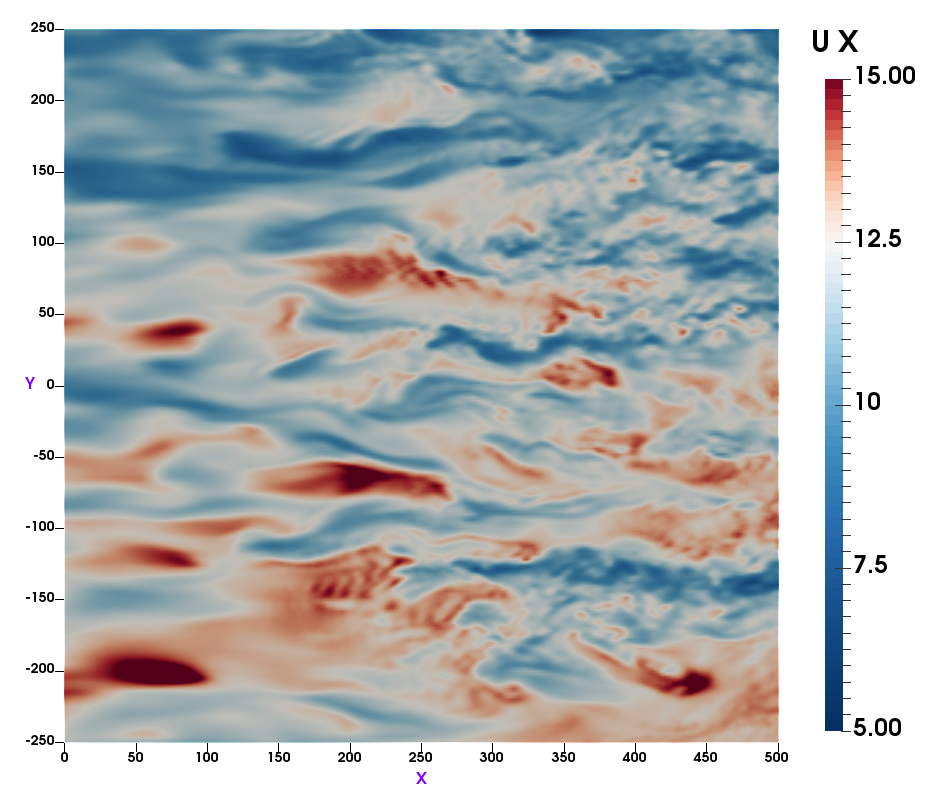
\includegraphics[width=0.45\textwidth]{FinePre/z=10m_UxSlice_17400.png}}
\caption{Instantaneous streamwise velocity in the coarse and fine precursor simulation at $Z_{agl} = 10 m$ plane.}
\label{fig:FP}
\end{figure}
% 
 
%\textcolor{red}{this statement is completley wrong. Think about it and reformulate. Consider specifying what should be expected first e.g. how the modeled and resolved contributions should change and how their sum should remain constant}


For any turbulent flow, a LES model shall yield the same ensemble-averaged resolved velocity profile for different grid resolution. As the grid gets finer in a LES, more turbulence scales get resolved and proportionally less sub-grid-scales (SGS) have to be accounted though the SGS stress model. Nevertheless, the total turbulence stress (resolved + SGS) profile for different simulation irrespective of grid resolution (i.e. filter size) shall remain consistent. The figure \ref{fig:PreComp} depicts the mean streamwise resolved velocity $\avT{\av{U}_x}$, streamwise normal stress $\SGSstress{u}{u}$ and shear stress $\SGSstress{u}{w}$ from both coarse precursor and fine precursor east-outlet boundary. Since the fine precursor domain width is much smaller than the coarse precursor, the velocity and stress fields corresponding to the fine precursor inlet dimension is considered only for comparison. The mean velocity profile $\avT{\av{U}_x}$ in figure \ref{fig:PreComp-U} obtained with the two levels of precursor simulation agree very well with each other and also agree well with the logarithmic law of the wall. 

%\textcolor{red}{This paragraph also needs improvement! You kept using ``terrain region'' or ``terrain surface'' this does not make sense in a flat precursor. Just call it the surface.}

In terms of the streamwise normal stress $\SGSstress{u}{u}$ (fig: \ref{fig:PreComp-uu}), the fine precursor SGS stress is smaller and resolved stress is larger compared to coarse precursor since more turbulent scales are resolved in the fine precursor. The total turbulence stress (resolved + SGS) matches well for both precursor simulations. A similar trend is also observed for the shear stress $\SGSstress{u}{w}$, except it is under-predicted at the near terrain region ($Z_{agl} \approx 10 m$) of the coarse precursor. Overall, the LES is consistent across both precursor simulations and the fine precursor contains desired smaller turbulent scales relevant to the Bolund hill height. Using such a sequential grid refining series of precursor simulations bridge the scale gap between atmospheric macro scales with near surface micro scales. It also requires much less computational resources than running only one large ABL precursor simulation with very fine resolution.

%
\begin{figure}[htb]
\centering   %%% not \center
	\subfloat[Streamwise mean resolved vel.$\avT{\av{U}_x}$]{\label{fig:PreComp-U}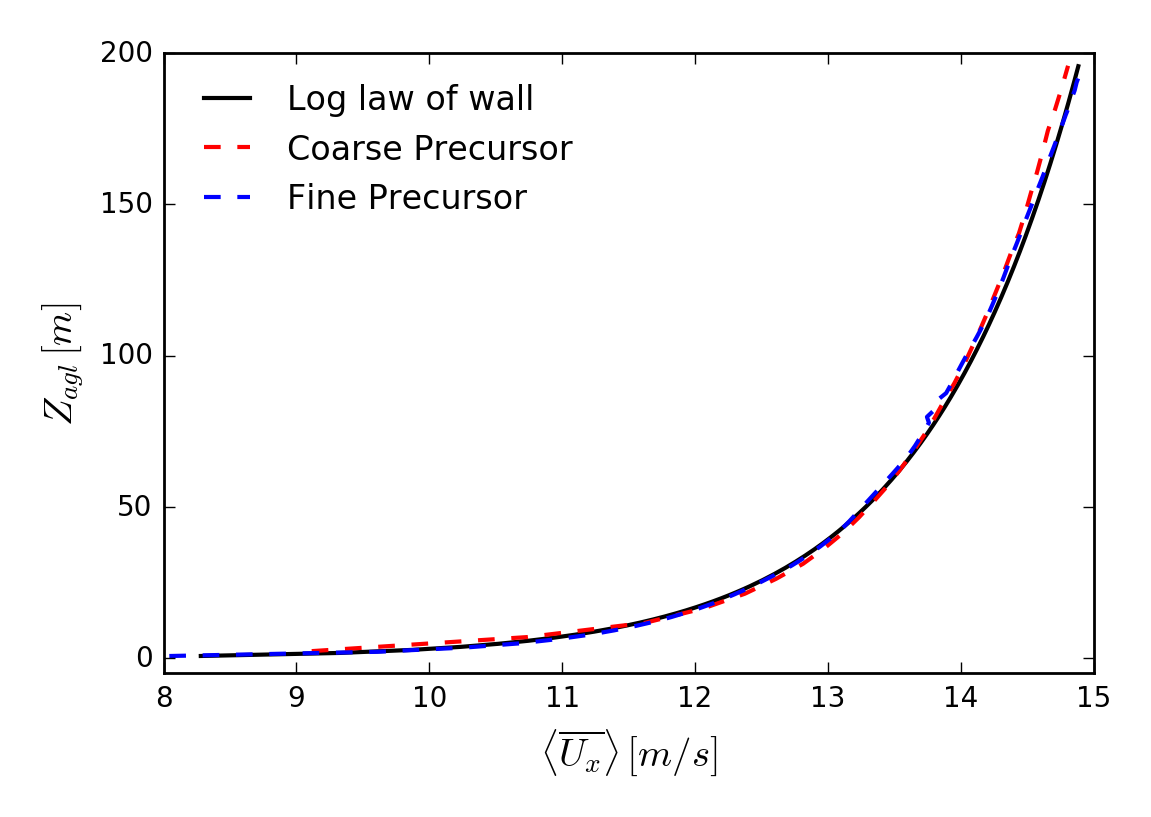
\includegraphics[width=0.32\textwidth]{CPvsFP/MeanVelocity.png}}
	%\quad
	\subfloat[Streamwise normal stress $\SGSstress{u}{u}$]{\label{fig:PreComp-uu}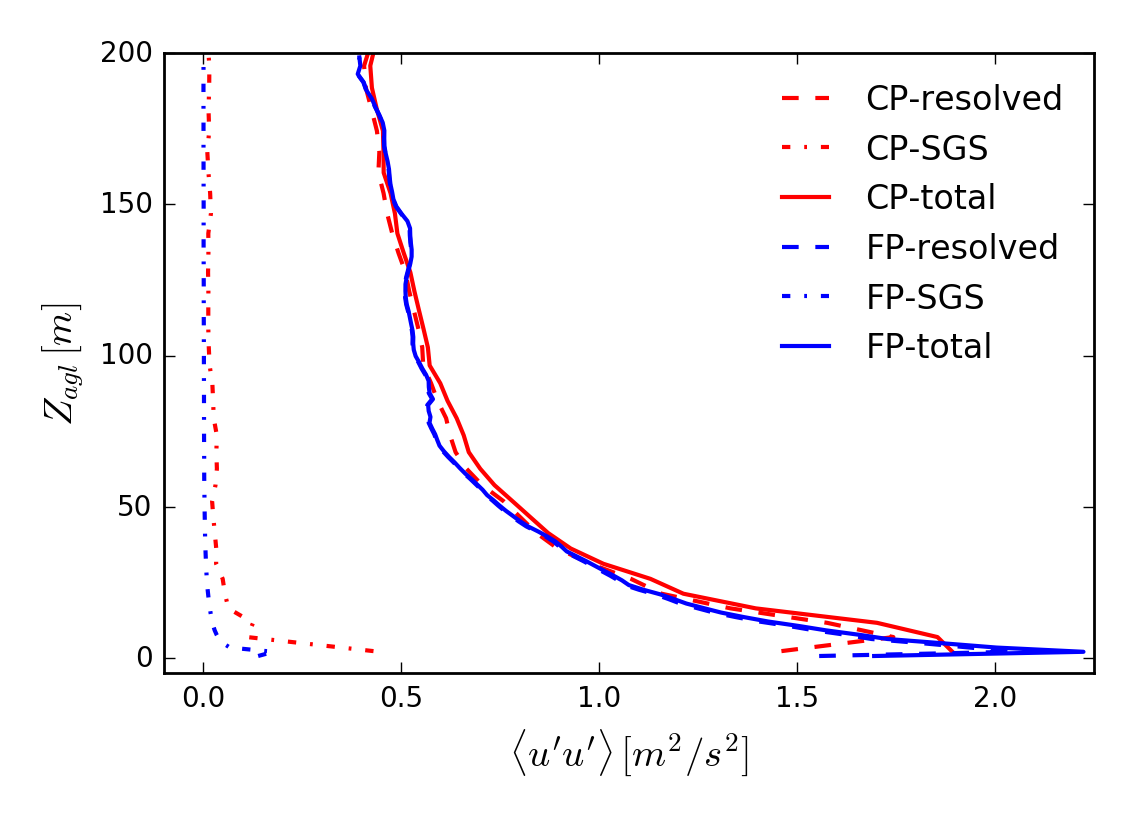
\includegraphics[width=0.32\textwidth]{CPvsFP/Stress-uu.png}}
	%\quad
	\subfloat[Vertical velocity $\SGSstress{u}{w}$]{\label{fig:PreComp-uw}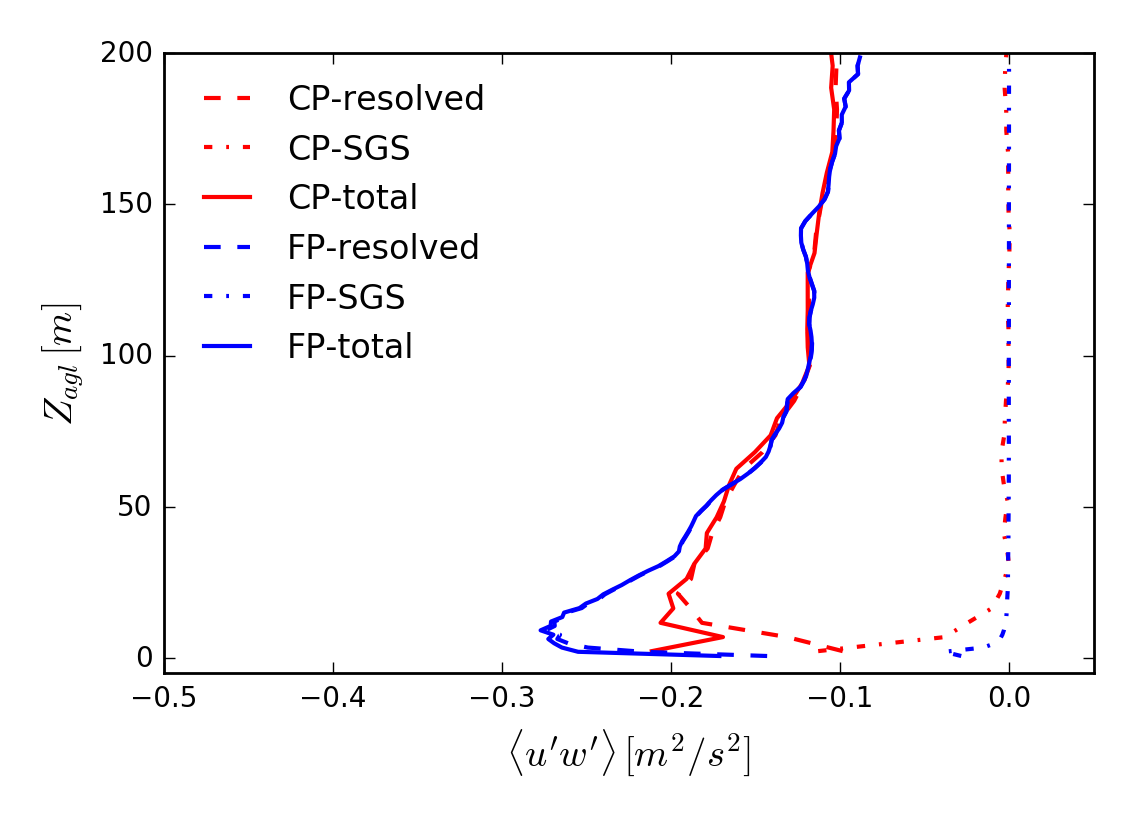
\includegraphics[width=0.32\textwidth]{CPvsFP/Stress-uw2.png}}
\caption{Mean velocity and stress comparison between coarse and fine precursor LES.}
\label{fig:PreComp}
\end{figure}
%

\subsection{Bolund Hill Simulation}
\label{subsec:5.2}
%
The computational domain considered for the Bolund hill simulation extends from $-300m$ upstream (west) to $400 m$ downstream (east) of the hill (i.e. $700m$ long in the wind-wise direction). In the crosswind direction, the domain extends from $-210m$ south to $190m$ north giving a total width of $400m$. These dimensions place the M0 and M9 masts sufficiently far from the domain boundaries. Both cross-wind boundaries are far enough from the hill to allow for streamline bending and flow evolution around the hill. The domain height is $120m$, which is about $11$ times of the maximum hill height and assumed to adequately represent the atmospheric boundary layer relevant to Bolund hill scale. The domain is aligned with the precursor domains, where the westerly wind is perpendicular to the west (inlet) boundary.
 
%
\begin{figure}[htb]
\centering   %%% not \center
	\subfloat[Terrain surface mesh]{\label{fig:surfMesh}\includegraphics[width=0.45\textwidth]{terrainMesh_wallSpacing7.png}}
	\quad
	\subfloat[Slice of volume mesh at $y=0 m$ plane]{\label{fig:volMesh}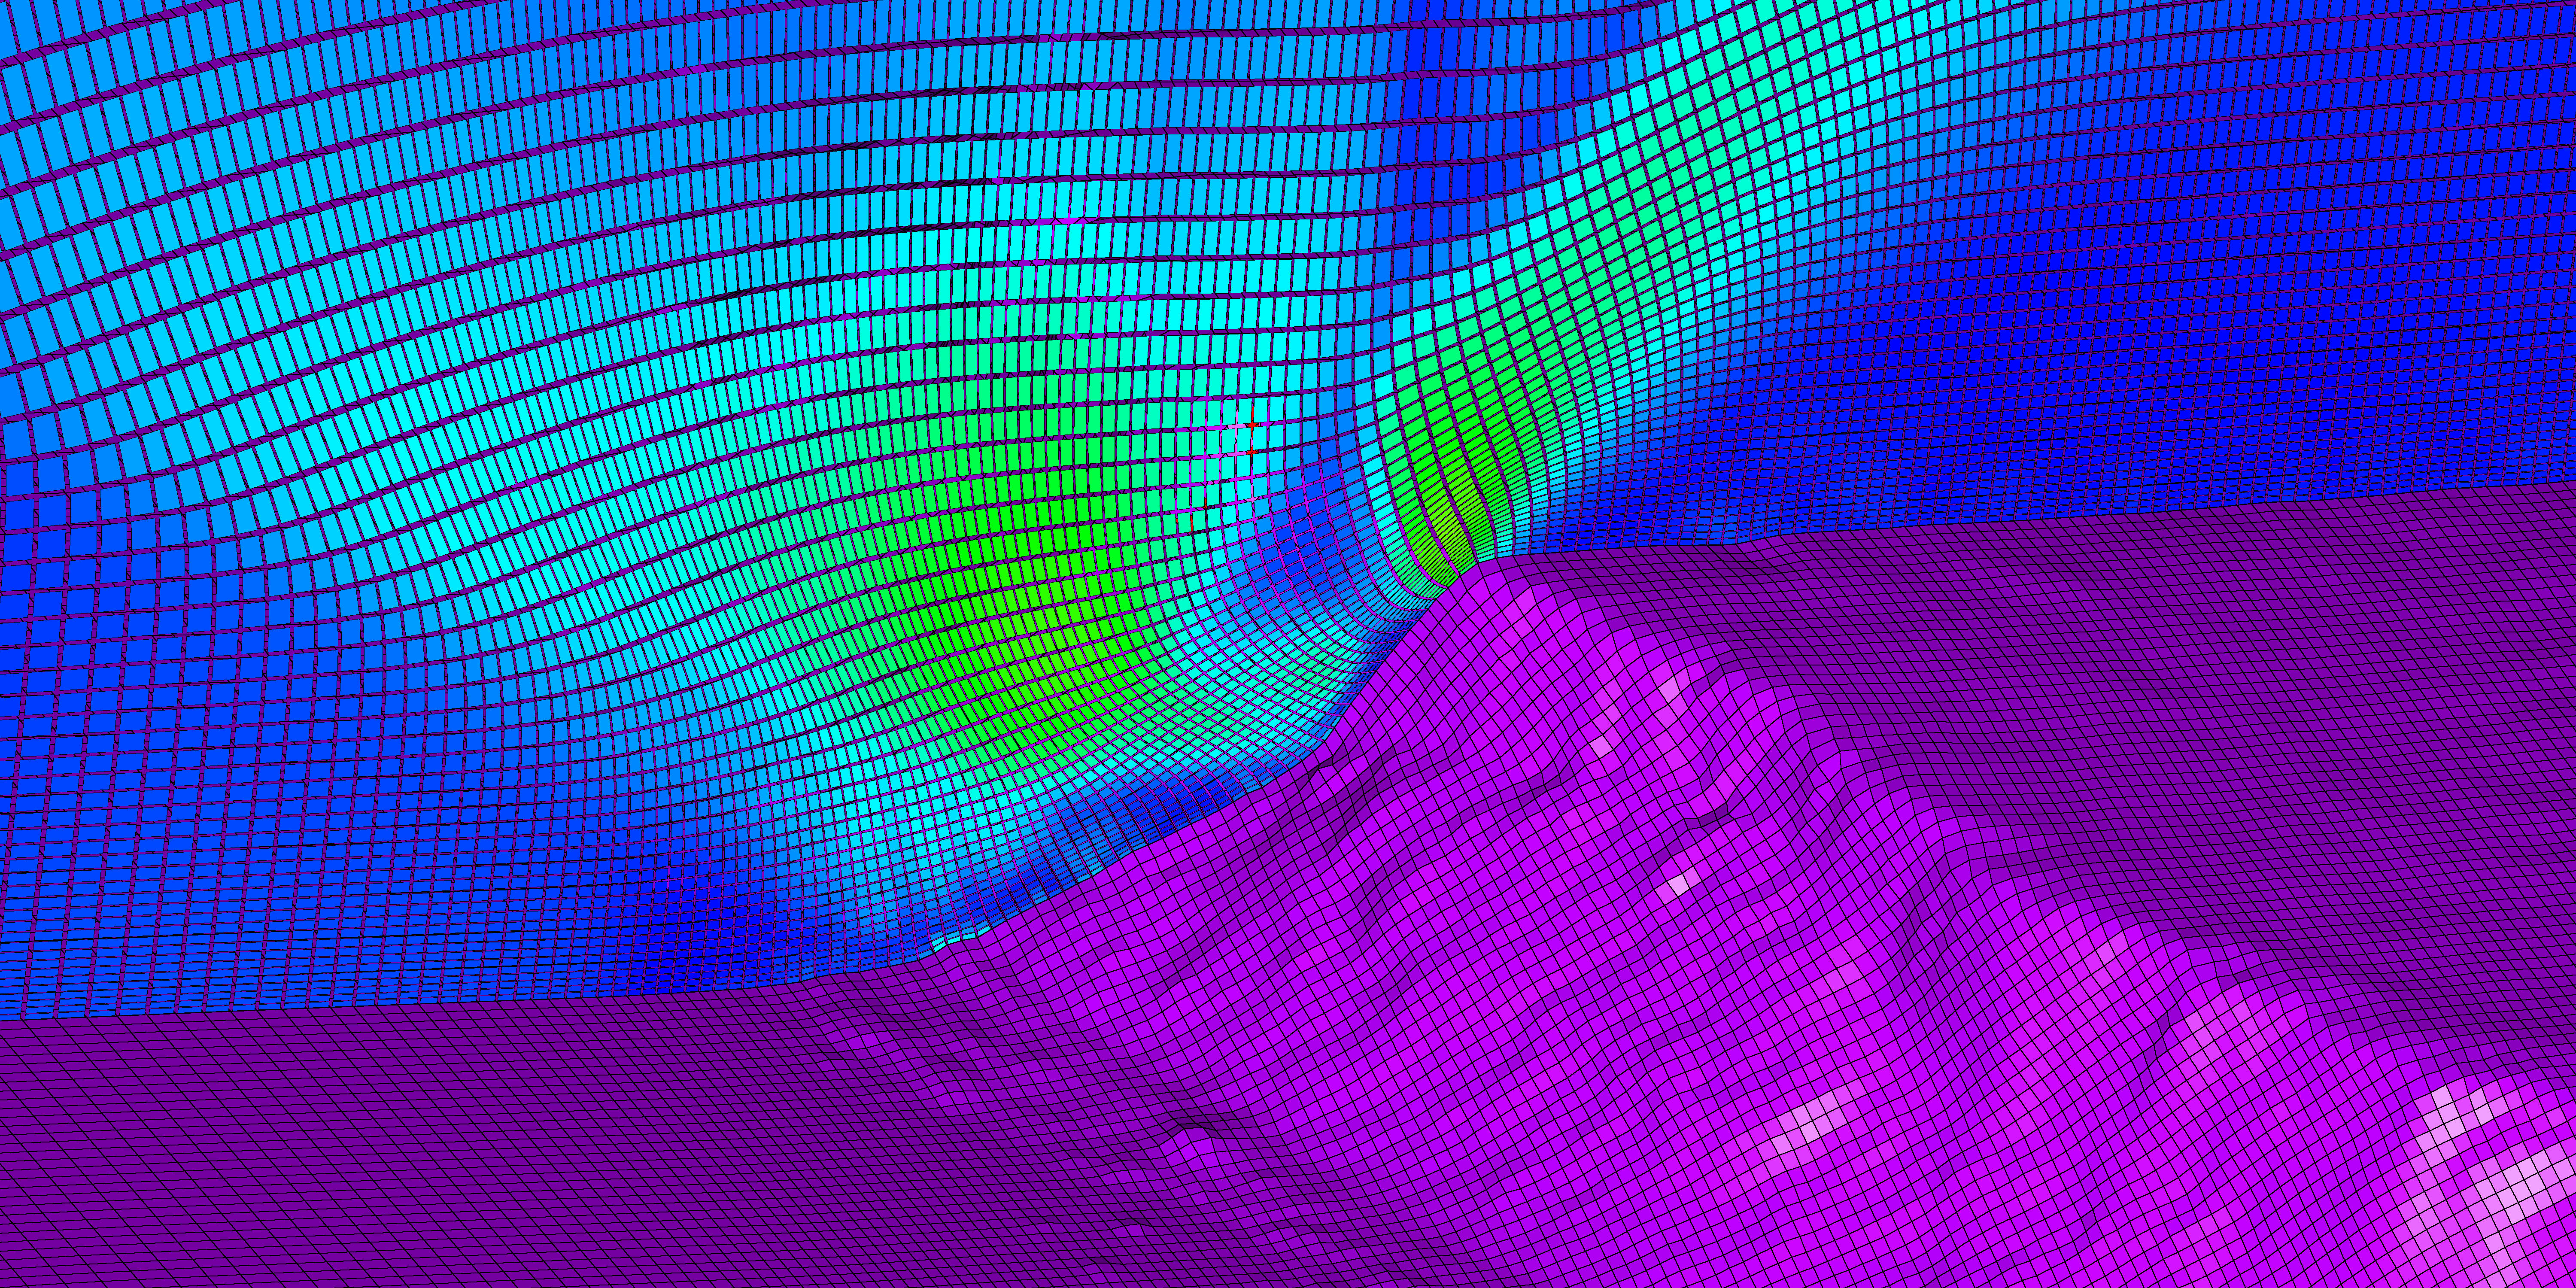
\includegraphics[width=0.45\textwidth]{maxAngle4.png}}
\caption{Mesh for Bolund hill simulation.}
\label{fig:HillMesh}
\end{figure}
%

An anisotropic hexahedral block-structured grid is prepared with the finest resolution of $\Delta x \approx 0.30 m$ and $\Delta y \approx 0.40m$ applied at the vertical escarpment. Over the rest of the hill surface, the horizontal grid spacing varies from $0.50 m \leq \Delta x, \, \Delta y \leq 0.75 m$ somewhat depending on the local terrain details. Beyond the hill, the grid is smoothly stretched to $\Delta x_{max}, \, \Delta y_{max} \approx 4 m$ at the domain boundaries. The near-terrain vertical grid resolution is set to $\Delta z_{terrain} \approx 0.15 m$ and smoothly stretched to $\Delta z_{max} \approx 5 m$ at the top boundary. Pointwise \cite{Pointwise}, a commercial software program, is used to prepare the terrain following multi-block structured mesh resulting in approximately $28 \times 10^6$ hexahedral cells. The figure \ref{fig:HillMesh} illustrates the structured surface mesh (fig. \ref{fig:surfMesh}) and a slice though the volume mesh at $y=0 m$ plane (fig. \ref{fig:volMesh}). Resolving the curvature at the vertical escarpment was challenging and a few moderately non-orthogonal cells are inevitably formed (marked by green color in fig. \ref{fig:volMesh}). The maximum non-orthogonality is around $138^o$ and the average is $5.7^o$. 

The Bolund hill surface roughness is prescribed as $z_{0,Bolund} = 0.015 m$, which is $25$ times higher than the calm bay water roughness of $z_{0,bay} = 0.0006 m$. Thus, the wind experiences a sharp transition of surface roughness (as well as shear stress) coupled with the complex geometric features (such as escarpment, steep slope, etc.) while blowing over the Bolund hill. In the east-outlet boundary a ``zero'' gradient Neumann condition for velocity and a fixed value ``zero'' Dirichilet condition for the modified pressure $p_{rgh}$ is prescribed. Slip-wall conditions for the velocity and ``zero'' gradient for all other variables are prescribed on the south, north and top boundaries. In the terrain surface, the Schumann-Grotzbach model is applied for wall shear stress and since the terrain is inhomogeneous a time average of the cell center velocity is used instead of the planar average used in the flat precursor simulations. 

%
\begin{figure}[htb]
\centering   %%% not \center
	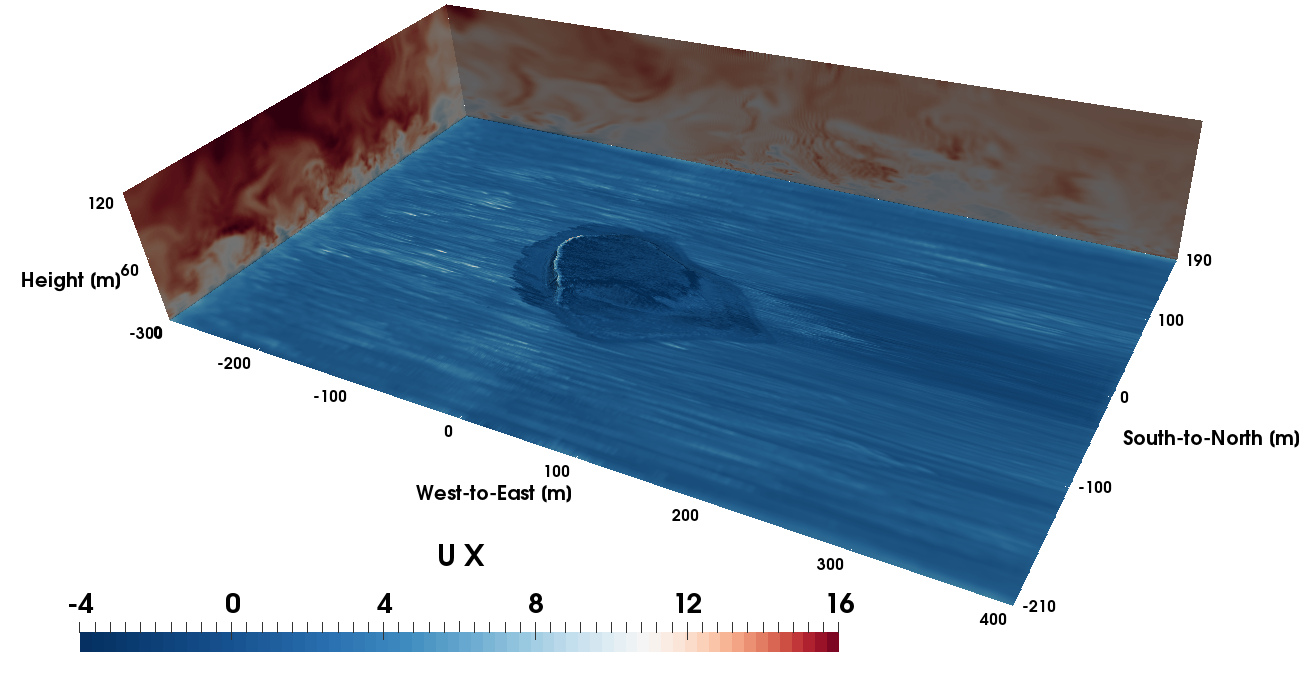
\includegraphics[width=0.65\textwidth]{Bolund/Ux_t17350_2.png}
\caption{Instantaneous streamwise velocity at the lower, west and north boundaries for the precursor inflow LES}
\label{fig:Bolund}
\end{figure}
%

To investigate the effect of inflow turbulence over the Bolund hill, two types of simulations are performed: i) steady inflow and ii) precursor inflow (turbulent). For the first case, a steady inflow velocity following the log-law of the wall is prescribed at the west-inlet boundary. In the second case, the spatio-temporally varying inflow velocity data generated in the fine precursor simulation is linearly interpolated to the west-inlet boundary during the simulation run-time. The surface velocities are modified following the procedure illustrated in figure \ref{fig:PreInterp} such that error from linear interpolation is minimized in the near surface region. All other variables are treated as ``zero'' gradient in the terrain boundary. The figure \ref{fig:Bolund} illustrates the instantaneous streamwise velocity field in the terrain, west and north boundaries for the precursor inflow simulation.

The \textit{ABLTerrainSolver} from the SOWFA library is used to execute the simulations. For the neutral atmospheric stability, a uniform potential temperature of $288 K$ is prescribed throughout the domain. To maintain stability, the solver has to operate at maximum allowed CFL number $0.9$, which resulted in time-step of $\Delta t \approx 5 \times 10^{-3} s$. To operate such a large computational domain with this minuscule time-step demands a considerable amount of time and computational resources. The width of the Bolund hill $100 m$ and the domain width $400 m$, which are much smaller than the width streaks observed in the coarse precursor. So multiple fine precursors and Bolund hill simulations recorded for a long time is necessary to investigate the influence of the atmospheric boundary layer characterized by long length and time scales.


However, considering enormous computational cost involved in such an endeavour, only one additional fine precursor and hill simulation is performed corresponding to a different window of the coarse precursor simulation. For both inflow cases, after an initial transient of $200s$ has passed, fields are only averaged over $600s$ each to gather flow statistics. The number of samples collected in the precursor inflow LES study are statistically inadequate compared to the numerous $600s$ datasets are considered in the experiment.


%For both inflow cases, after an initial transient of $200s$ has passed, flow statistics are gathered over $600 s$ only mainly due to computational resource limitation. Since the spatial and temporal scales of the atmospheric boundary layer can be very large, simulating with a short time of the precursor inflow does not represent the wide variety of the ABL scales. In fact, following the experimental campaign, numerous $600s$ simulations shall be conducted with turbulent inflow from vastly different times. Considering enormous computational cost involved in such an endeavor, only one additional fine precursor and hill simulation is performed corresponding to a different window of the coarse precursor simulation.  
 
%
\begin{figure}[!htb]
\centering   %%% not \center
	\subfloat[Mean velocity magnitude]{\label{fig:M0-U}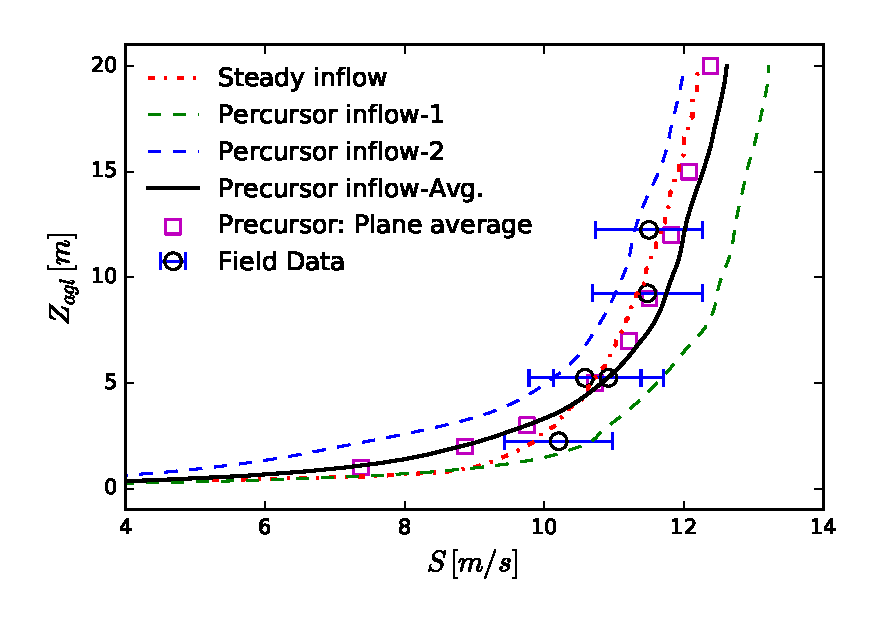
\includegraphics[width=0.46\textwidth]{velProfiles-wSTD/AvgVelProfileatProbe_M0_infloPln.eps}}
	\quad
	\subfloat[Turbulence Kinetic Energy]{\label{fig:M0-TKE}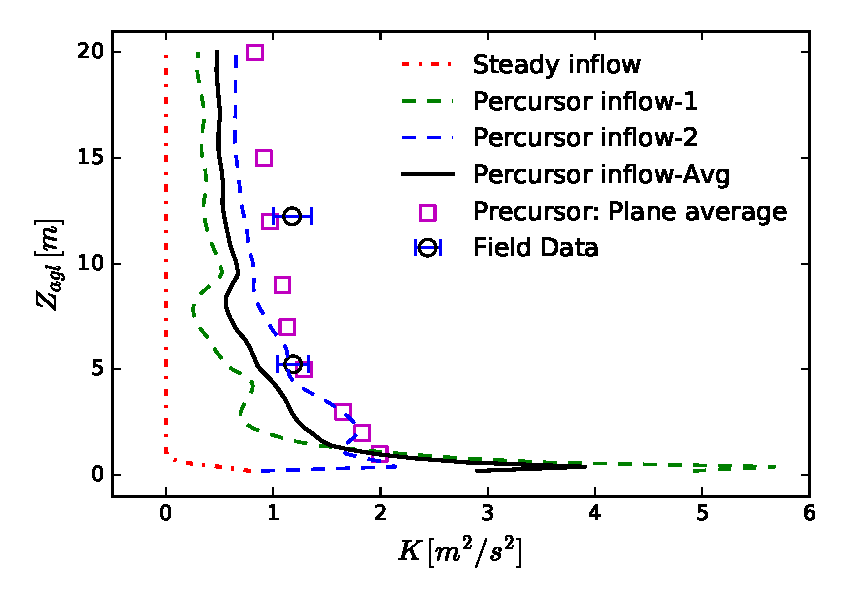
\includegraphics[width=0.44\textwidth]{stressProfiles-wSTD/TKE_M0_infloPln.eps}}
\caption{Mean wind speed $S$ and Turbulence Kinetic Energy $K$ at the inflow mast $M0$.}
\label{fig:M0}
\end{figure}
%

%\textcolor{red}{Please work on this section some more!}

In figure \ref{fig:M0}, the mean wind-speed $S$ and Turbulence Kinetic Energy (TKE) $K$ profiles are depicted for both steady and precursor inflow cases at the inflow Mast $M0$. The difference of the mean velocity profile between the precursor inflow simulations emphasises the need for statistics from more LES. To fill the vacancy of inadequate, the mean wind speed values are further averaged along the mast $M0$ plane ($x=-181.3 m$) at different height levels which agrees very well with field data \ref{fig:M0-U}. The mean wind speed profile from the steady inflow LES is also in good agreed with field measurements.

In the TKE plot (fig. \ref{fig:M0-TKE}), fluctuations in the precursor-inflow profiles denotes the inadequate averaging time. Significant TKE variations, particularly at the near surface region, is observed for two precursor inflow cases. However, the planer average ($x=-181.3 m$) profile for both precursor simulations and the steady inflow profile both agrees very well with the field data. The steady inflow produces negligible TKE $K$, as expected. 
%
\begin{figure}[!htb]
\centering   %%% not \center
	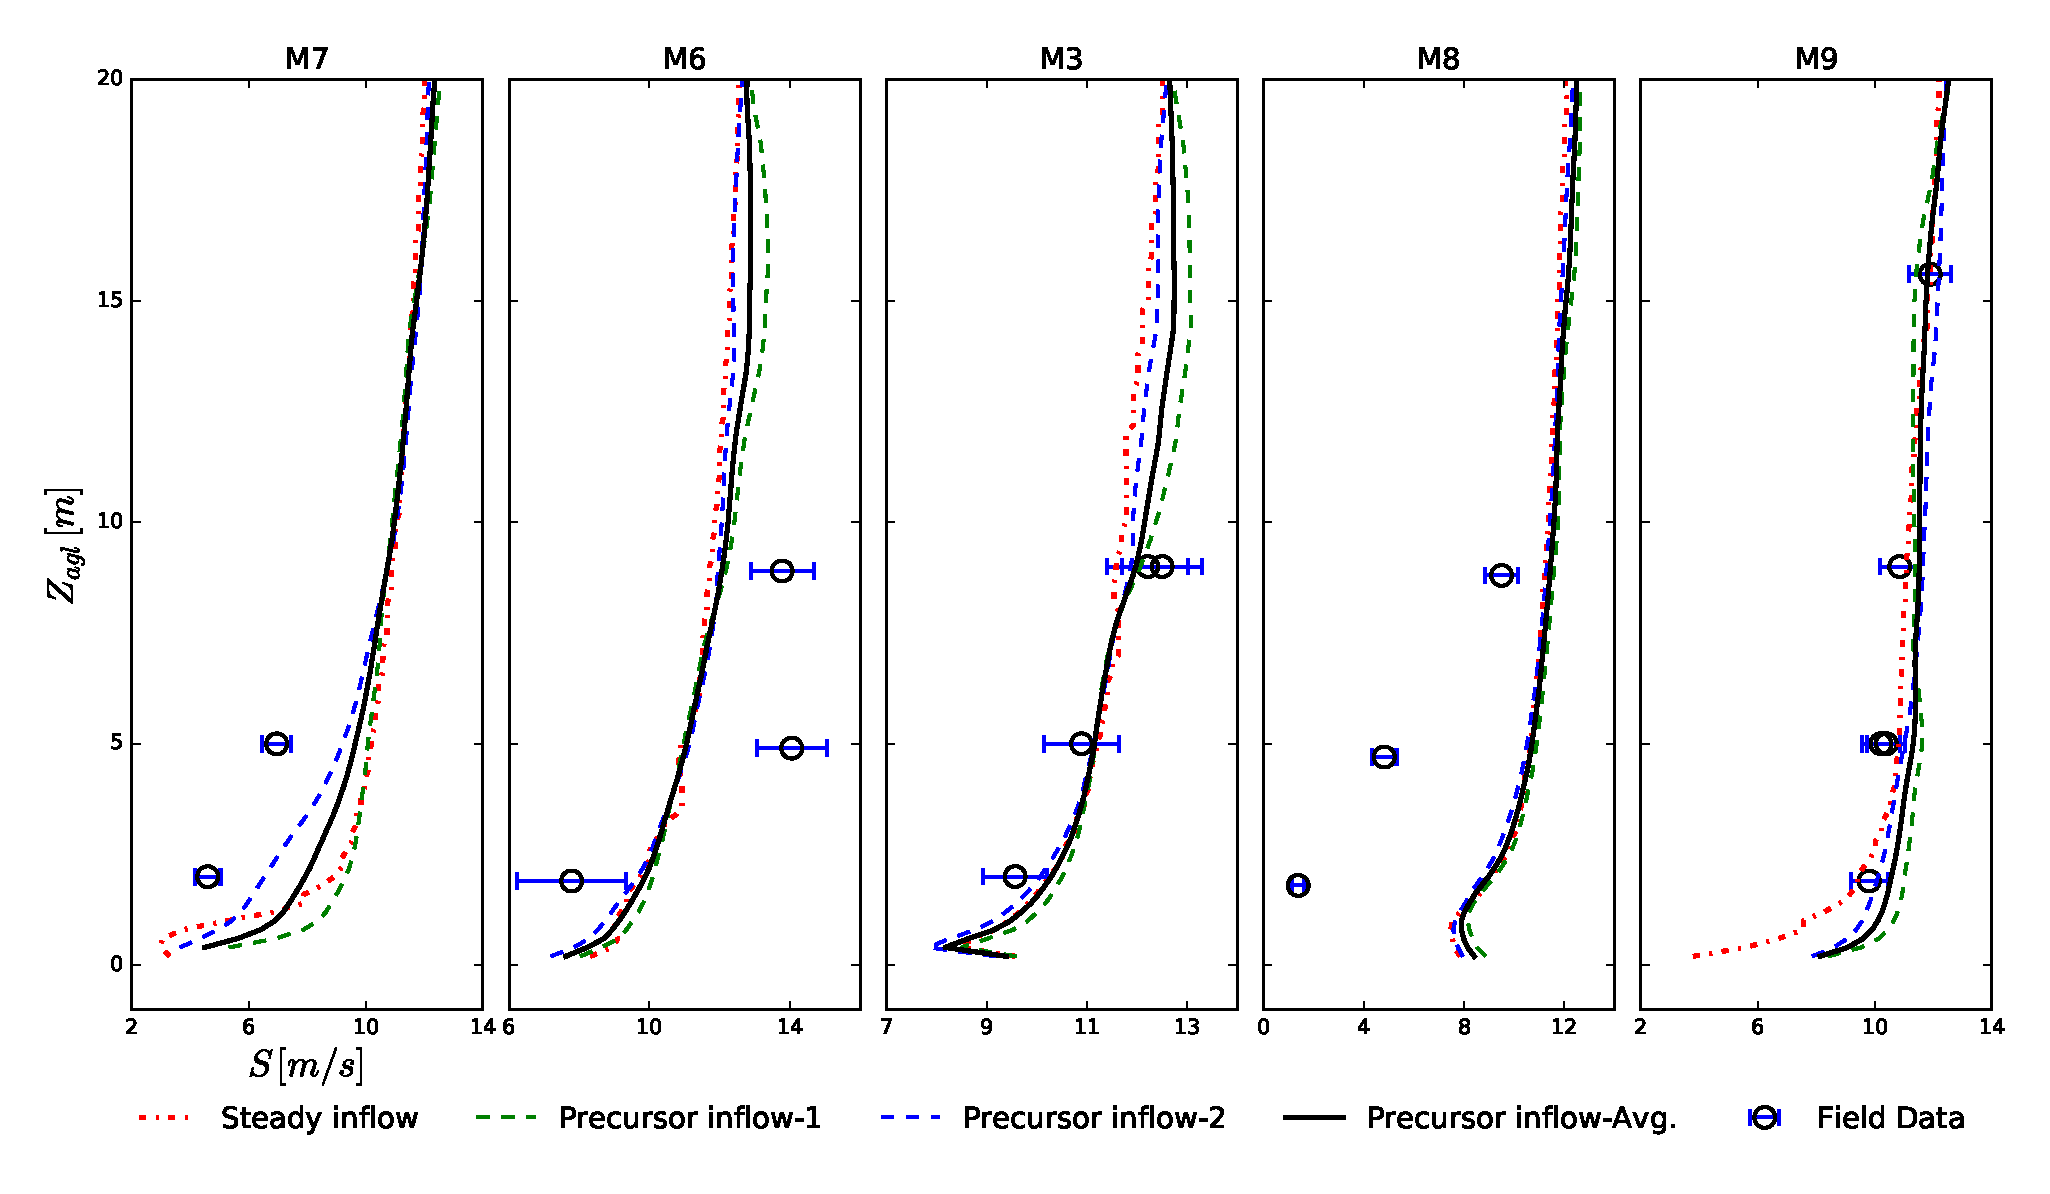
\includegraphics[width=0.95\textwidth]{velProfiles-wSTD/Vel_lineB.eps}
\caption{Mean streamwise velocity comparison at multiple heights for measurement masts $M7, \,M6, \,M3, \,M8$ and $M9$.}
\label{fig:velLineB}
\end{figure}
%

Illustrated in the figure \ref{fig:contour}, the masts $M7, \,M6, \,M3, \,M8$ and $M9$ are aligned perpendicular to the westerly wind flow. The $M7$ located at the western foothill of the near-vertical escarpment, $M6$ on the ridge, $M3$ in in the center of the hill, $M8$ on the eastern foothill and $M9$ is in the downstream wake. Here, each of mast characterizes near surface wind profiles in different regions of the boundary layer flow. The figure \ref{fig:velLineB} depicts the mean wind profile at these five mast locations. 

Surprisingly, the mean wind profile of the steady inflow case shows only minor deviation from the precursor inflow cases. Wind profile predicted in the mast $M3$ and $M9$, which are placed in nearly flat terrain, are well predicted for both steady and precursor inflow cases. The most deviation occurs at near the foothill masts ($M7$ and $M8$) for both inflow cases. The simulated wind experienced rapid acceleration over the western escarpment (near $M7$), but slower declaration at the eastern steep slope (near $M8$). Overall, largest deviation usually occurred at the bottom-most probe and the prediction accuracy proportionally improves with the height above ground.
%
\begin{figure}[!htb]
\centering   %%% not \center
	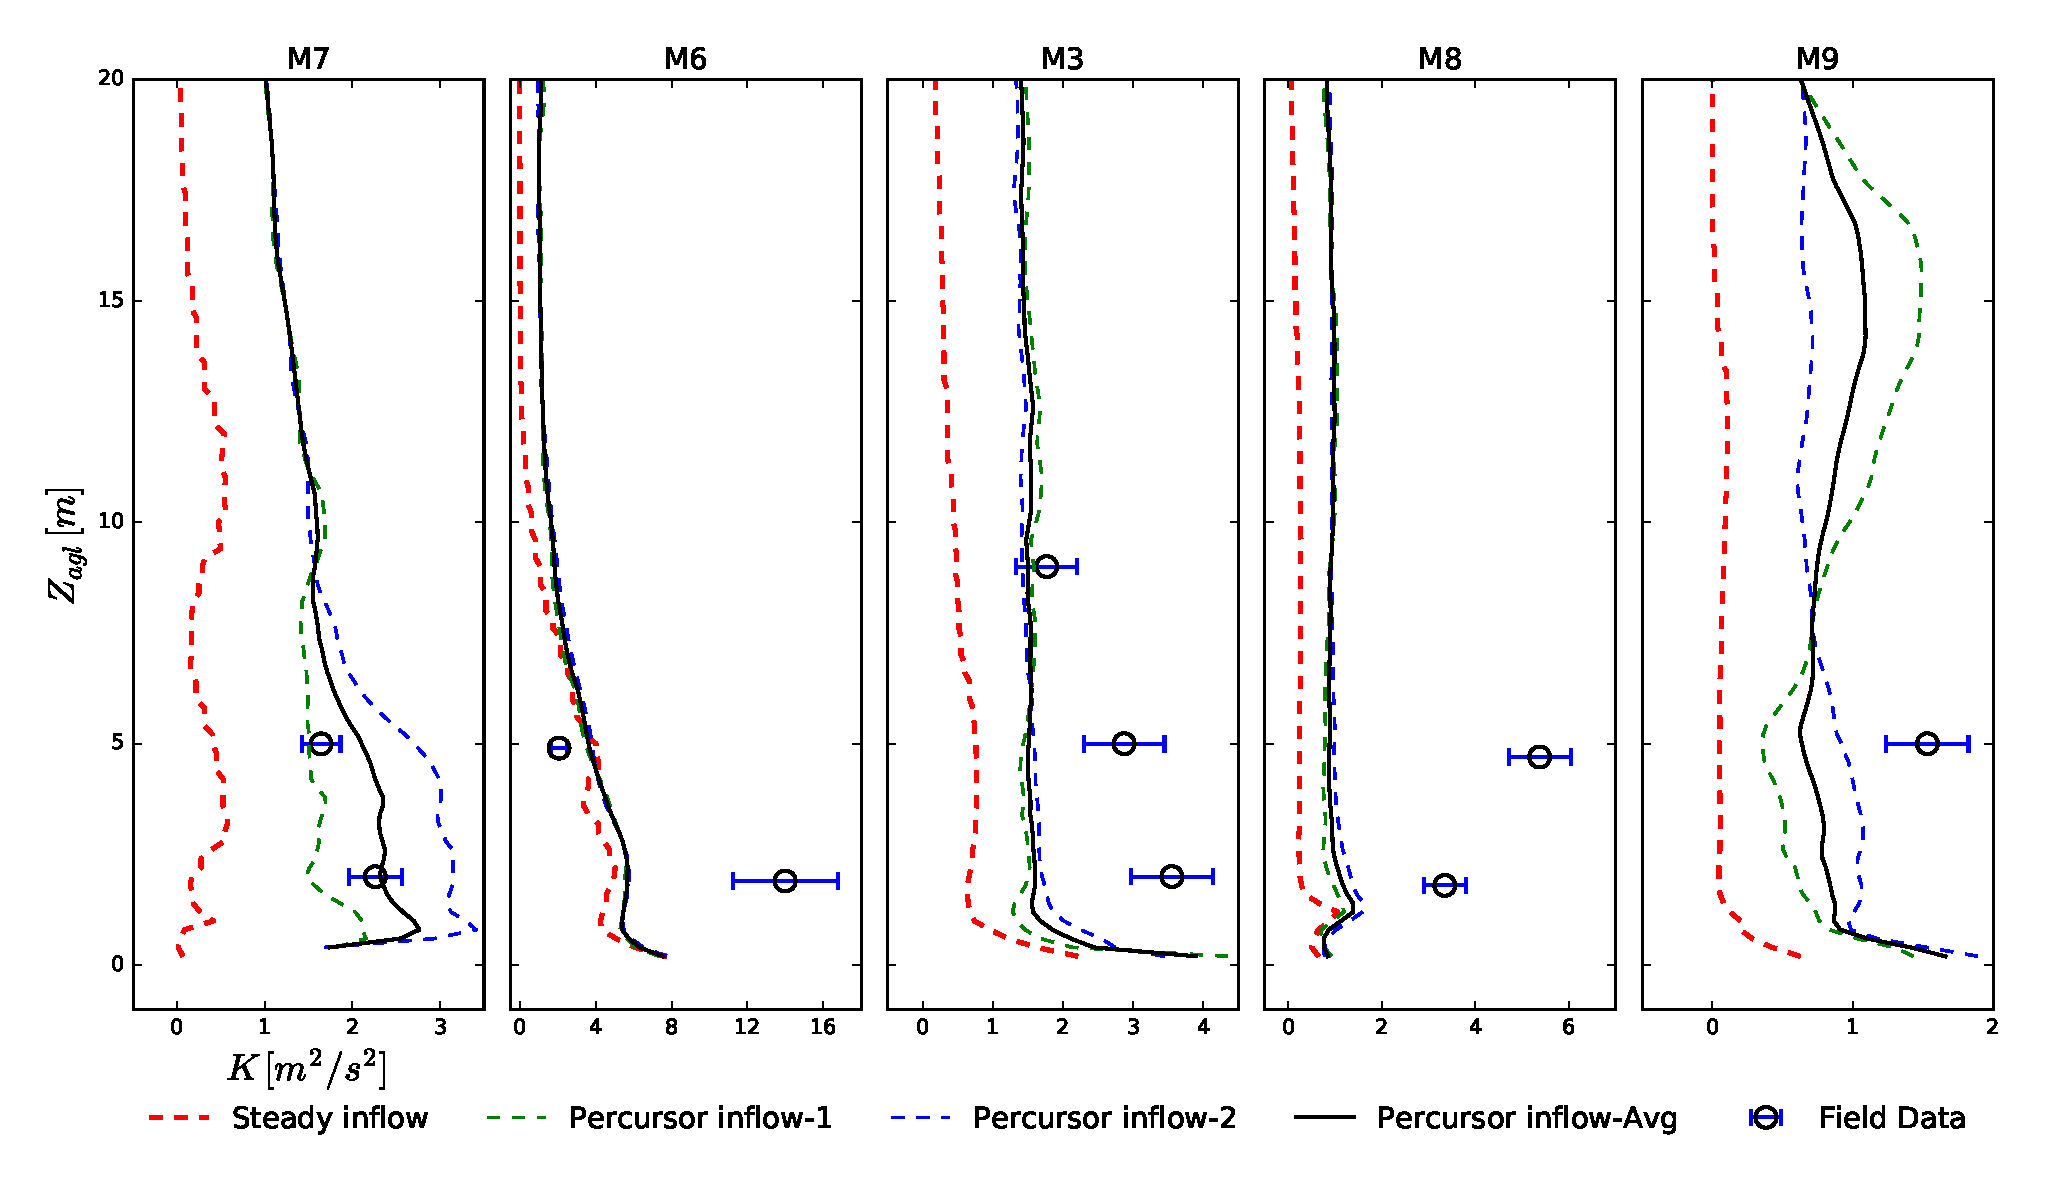
\includegraphics[width=0.95\textwidth]{stressProfiles-wSTD/TKE_lineB.eps}
\caption{Turbulence kinetic energy comparison at multiple heights for measurement masts $M7, \,M6, \,M3, \,M8$ and $M9$.}
\label{fig:TKELineB}
\end{figure}
%
The figure \ref{fig:TKELineB} illustrates the TKE profiles for these five masts. For the steady inflow case, TKE is under-predicted in every mast locations. In the two precursor inflow cases, deviation in the TKE values at the mast $M7$ and $M9$ signifies influence of different turbulent inflow. Similar to mean wind profile, TKE is better predicted at the flat terrain masts ($M3$ and $M9$) and poorly predicted in rest of the masts ($M7$, $M6$ and $M8$). At the western-foothill (upstream) mast $M6$, TKE is under-predicted near the surface, which also shows near surface over-prediction of velocity. Overall TKE is under-predicted for both precursor cases. 
%
%
%

%\section{Summary}
%\label{sec:6}
%\textcolor{red}{I don't think you need a summary. Just focus on the conlcuisons}
%To investigate the wind flow over complex terrain, large eddy simulation (LES) of atmospheric boundary layer flow over the Bolund hill is investigated and compared against the field measurements. The effect of Coriolis force is neglected due to small height of the hill compared to the boundary layer depth. The wind flow is assumed incompressible and Boussinesq buoyancy assumption is used to account for the temperature fluctuation induced buoyancy. SOWFA, a solver library based on the OpenFOAM solver, is used as the LES model. For ease of simulation, only westerly wind $270^o$ and neutral atmospheric stability condition are considered.
%
%The effects of turbulent inflow are investigated with two types of simulation: i) with steady inflow and ii) time varying inflow. For the later case, a coarse precursor simulation is performed in a flat homogeneous terrain and velocity fields are recorded at the outlet boundary to build an inflow library. In the coarse precursor, presence alternate high and low-velocity streaks are observed extending the entire streamwise domain. Due to short domain length, these long streak structures can't get decorrelated and longer domain length shall be used.
%
%Since the grid resolution in the coarse precursor is large $5-15 m$ compared to the Bolund hill height $h = 11m$, another precursor with finer resolution $1-4 m$ is performed, where inflow fields from the coarse precursor are prescribed in the inlet boundary. Similar to the coarse precursor, outflow velocities from the fine precursor are recorded, which are later fed into the Bolund hill LES. During the sequential precursor simulation process, the mean wind speed, normal stress, and shear stress conservation are maintained except small shear-stress deviation is observed at near surface between coarse and fine precursor.
%
%\textcolor{red}{This shoild go into the result section?}
%The width of the Bolund hill $100 m$ and the domain width $400 m$, which are much smaller than the width streaks observed in the coarse precursor. So multiple fine precursors and Bolund hill simulations recorded for a long time were necessary to investigate the influence of the atmospheric boundary layer characterized by long length and time scales. However, due to computational resource limitation, only two LES were performed and fields are only averaged over $600s$ each to gather flow statistics. The number of samples collected in this study are statistically inadequate compared to the numerous $600s$ datasets are considered in the experiment.
%
%At the inflow mast $M0$, mean wind speed from the steady inflow and precursor inflow (planner average) cases agrees well with the field data. However, the turbulence kinetic energy (TKE) is near ``zero'' for the steady inflow, but the precursor inflow is in good agreement with the field data. Over the Bolund hill, the velocity, and TKE profiles are compared for the masts $M7, \,M6, \,M3, \,M8$ and $M9$, which are aligned with the streamwise direction. In terms of mean wind speed, the velocities are well predicted in the relatively flat regions ($M3$ and $M9$). In the masts at the foothills ($M7$ and $M8$), the simulated wind experiences rapid acceleration over the western escarpment, but slower declaration at the eastern steep slope. It seems that the LES model prescribes smaller shear stress in these complex geometric regions.
%
%In the steady inflow case, TKE is nearly zero except very close to the surface and mostly under-predicted. It underscores the importance of turbulent inflow in LES of complex terrains. In the cases of precursor inflow, the TKE is under-predicted, but prediction improved as height above the ground increases. Over the mast $M6$ at $2m$ height above the ridge, the TKE is highly under-predicted which also explains over-prediction of the wind speed. 


\section{Conclusions}
\label{sec:6}
Large eddy simulations of wind flow over the Bolund hill are performed for neutrally stable atmospheric boundary layer flow and validated with field measurements. Influence of inflow boundary condition is investigated for steady and precursor LES derived inflow types. To bridge the turbulence scale gap between very large atmospheric macro scales and near surface micro scales, a series of coarse and fine precursor LES are performed in sequence. The mean resolved wind speed and total turbulence stress (resolved + sub-grid-scale) profiles are found consistent across the precursor simulations. In the coarse precursor, the presence of very large streaks engulfing the entire streamwise extension was observed. The streamwise extension of the domain needs to be increased to allow for decorrelation of such long structures. In the fine precursor, the evolution of smaller turbulent scales has happened within a short span. The sequential precursor LES approach is appeared as an optimal and feasible approach to generate realistic turbulent inflow for LES.

Assessing the influence of inflow boundary, the steady inflow case under-predicted the turbulence kinetic energy in almost every mast locations, which underscores the importance of applying turbulent inflow in complex terrain LES. Due to computational resource limitation, the precursor inflow LES was performed for two separate inflow fields for 10 minutes each, hence the statistics collected is inadequate compared to plenty of 10 minutes datasets are collected in the field experiment. The precursor inflow LES demonstrated good match with reference inflow reference mast measurements. Over the hill, the LES model performed well in the relatively flat terrain and wake regions but underperformed in complex geometric regions such as escarpment, ridge, steep slopes, etc. The reason for deviation is not clear but encourages to further investigation in few key areas of the simulation.

The ``Slip'' boundary condition applied in the lateral and top boundaries is far from ideal and caused additional flow acceleration over the hill which can affect both mean wind and TKE profiles. Better boundary condition shall be applied which allows inflow and outflow across these boundaries. The 10 minute average of the precursor inflow bears significant variations in the lateral direction due to the presence of the very long streaks. Influence of turbulence in the inflow boundary is realized in the case of steady inflow, thus a more accurate precursor inflow field needs to be prepared. Flow over complex terrain features such as escarpment, steep slopes, etc. is characterized by the presence of strong pressure gradient, thus doesn't follow the logarithmic law of wall. An more appropriate wall model for surface shear stress for complex terrain has to be implemented in the LES model.

Overall, a sequential precursor approach is developed to generate realistic turbulent inflow for LES of complex terrains and the Bolund hill LES with precursor inflow demonstrated some success in the flat terrain regions. Few modifications in the numerical model, precursor domain setup (as mentioned in the preceding paragraphs) will be implemented in the future works. 


\section*{Acknowledgements}
This work was supported by the U.S. Department of Energy, Office of Science, Basic Energy Sciences, under Award \# DE-SC0012671. We would like to acknowledge the use of computational resources (ark:/85065/d7wd3xhc) at the NCAR-Wyoming Supercomputing Center provided by the National Science Foundation and the State of Wyoming, and supported by NCAR's Computational and Information Systems Laboratory \cite{NCAR_CISL}. We also acknowledge the research computing support we have received from the Advanced Research Computing Center (ARCC) at the University of Wyoming. The authors highly acknowledge the Bolund experimental campaign team, especially Andreas Bechmann for providing the field measurement datasets and Bolund hill terrain geometric information. We would like to also acknowledge the NREL for providing the open source SOWFA package online.
%